\chapter{ادراک شنیداری، مقیاس مل و ضرایب \eng{MFCC}}

در جلسات پیشین، سیگنال گفتار را از دید فیزیکی و آکوستیکی بررسی کردیم: شکل موج، تبدیل فوریه، هارمونیک‌ها، فرمنت‌ها، فضای واکه‌ای و رابطهٔ ویژگی‌های تولیدی با ویژگی‌های آکوستیکی. در همهٔ آن تحلیل‌ها با طیفی سروکار داشتیم که همهٔ فرکانس‌ها را به یک چشم می‌دید. در این جلسه یک گام جلوتر می‌رویم: ویژگی‌های \term{سیستم شنوایی انسان}{Human Auditory System} را وارد فرایند استخراج ویژگی می‌کنیم. حاصل این کار مقیاس مل، بانک فیلتر مل، لگاریتم‌گیری از انرژی‌ها و در نهایت \term{ضرایب کپسترال فرکانس مل}{Mel-Frequency Cepstral Coefficients} یا به‌اختصار \eng{MFCC} است؛ ویژگی‌ای که تا امروز در بخش بزرگی از سامانه‌های گفتاری به کار می‌رود و در جلسات بعد نیز بارها به آن بازخواهیم گشت.

\begin{exambox}{نقشهٔ راه جلسه}
مسیر منطقی جلسه به این صورت است: (۱) چرا باید شنوایی انسان را مدل کنیم؟ (۲) نقشهٔ تونوتوپیک حلزون گوش و مرور \eng{Praat}؛ (۳) مقیاس مل و بانک فیلتر مثلثی؛ (۴) لگاریتم برای ادراک غیرخطی بلندی؛ (۵) افزونگی ویژگی‌ها و تبدیل کسینوسی گسسته (\eng{DCT}) و پیدایش ضرایب \eng{MFCC}؛ (۶) روایت تاریخی کپستروم؛ (۷) کاربردها و رابطهٔ \eng{MFCC} با یادگیری ماشین و یادگیری عمیق.
\end{exambox}

%====================================================================
\section{چرا باید ادراک شنیداری انسان را در نظر بگیریم؟}
%====================================================================

تا اینجا، تبدیل فوریه به ما می‌گفت هر مؤلفهٔ فرکانسی چه سهمی در سیگنال دارد، بدون آنکه بپرسد انسان کدام فرکانس‌ها را بهتر تشخیص می‌دهد. اما سیستم شنوایی انسان همهٔ فرکانس‌ها و همهٔ شدت‌ها را یکسان پردازش نمی‌کند. اگر بخواهیم سامانه‌ای بسازیم که رفتارش به ادراک انسان نزدیک باشد (و در عمل، چون گفتار برای شنیده‌شدن توسط انسان تکامل یافته است، بیشترِ اطلاعات مهم آن در همان محدوده‌هایی است که گوش به آن‌ها حساس است)، باید محدودیت‌ها و ویژگی‌های شنوایی را بشناسیم.

\subsection{محدودهٔ شنوایی}
انسان جوان و سالم معمولاً صداهایی را در محدودهٔ تقریبی \textbf{۲۰ هرتز تا ۲۰ کیلوهرتز} می‌شنود. فرکانس‌های پایین‌تر از این محدوده (مادون‌صوت) و بالاتر از آن (فراصوت) به‌صورت صدا ادراک نمی‌شوند. اما نشنیدن یک ارتعاش به معنای نبودن آن نیست؛ برای نمونه ممکن است یک ارتعاش مکانیکی شدید را با بدن احساس کنیم بی‌آنکه آن را «بشنویم». پس دو چیز را باید از هم جدا کرد:
\begin{itemize}
  \item \textbf{وجود فیزیکی ارتعاش}: پدیده‌ای که طبق قوانین فیزیک رخ می‌دهد.
  \item \textbf{ادراک شنیداری ارتعاش}: فرایندی که طی آن ارتعاش از بخش‌های مختلف دستگاه شنوایی می‌گذرد و در نهایت در مغز پردازش و به تجربهٔ شنیدن تبدیل می‌شود.
\end{itemize}

برای روشن‌شدن این تفاوت می‌توان به سیستم بینایی مراجعه کرد. اگر چراغی با فرکانس مشخصی چشمک بزند، روشن‌وخاموش‌شدن آن را می‌بینیم؛ اما اگر فرکانس چشمک‌زدن بسیار زیاد شود، دیگر چشمک‌های جداگانه را تشخیص نمی‌دهیم و چراغ را پیوسته روشن می‌بینیم، هرچند از نظر فیزیکی همچنان خاموش و روشن می‌شود. سیستم شنوایی نیز محدودیت‌های مشابهی دارد.

\begin{exambox}{نتیجهٔ کلیدی}
در پردازش گفتار، دانستن مشخصات فیزیکی سیگنال کافی نیست؛ باید بدانیم انسان این مشخصات را \emph{چگونه درک می‌کند}.
\end{exambox}

\begin{addedbox}{محدودهٔ شنوایی و گفتار}
محدودهٔ ۲۰ هرتز تا ۲۰ کیلوهرتز مربوط به شنوندهٔ جوان است و با افزایش سن (بخش \ref{sec:presbycusis}) حد بالایی آن پایین می‌آید. بیشترِ انرژی و اطلاعات گفتار در زیر حدود ۸ کیلوهرتز قرار دارد؛ به همین دلیل در سامانه‌های تشخیص گفتار معمولاً با نرخ نمونه‌برداری \eng{16 kHz} کار می‌کنند (طبق قضیهٔ نایکوییست، فرکانس‌ها تا ۸ کیلوهرتز را نمایش می‌دهد) و در تلفن سنتی با \eng{8 kHz} (فرکانس‌ها تا ۴ کیلوهرتز؛ پهنای باند مؤثر خط تلفن حدود ۳۰۰ تا ۳۴۰۰ هرتز است).
\end{addedbox}

%====================================================================
\section{نقشهٔ تونوتوپیک حلزون گوش}
%====================================================================

برای فهم چگونگی پردازش فرکانس در گوش، باید به گوش داخلی و بخش مهم آن یعنی \term{حلزون گوش}{Cochlea} نگاه کنیم. صدا پس از عبور از گوش خارجی و میانی، از طریق دریچهٔ بیضی (\eng{oval window}) به مایع درون حلزون منتقل می‌شود و در درون حلزون موجی روی \term{غشای پایه}{Basilar Membrane} پدید می‌آید. نکتهٔ مهم این است که نقاط مختلف این غشا به فرکانس‌های مختلف حساس‌اند. به این سازمان‌دهی فرکانسی، \term{نقشهٔ تونوتوپیک}{Tonotopic Map} می‌گویند (از ریشهٔ \eng{tonos} به معنای «آهنگ/نغمه» و \eng{topos} به معنای «مکان»).

\begin{figure}[htbp]
  \centering
  \fbox{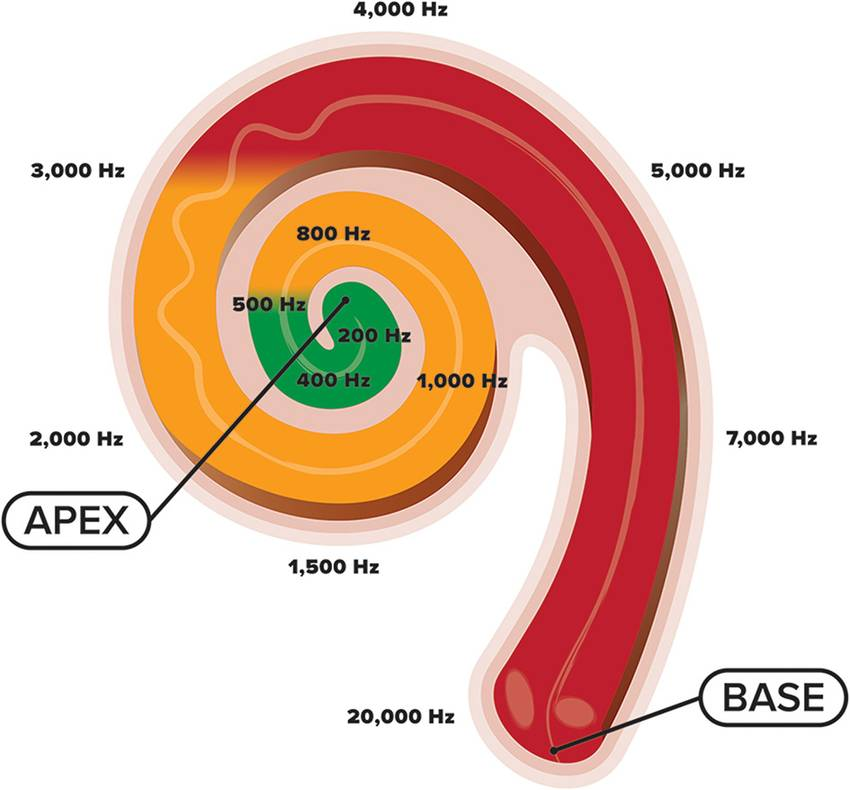
\includegraphics[width=0.46\textwidth]{../assets/figures/ch05-cochlea-tonotopic.png}}\hspace{0.03\textwidth}
  \fbox{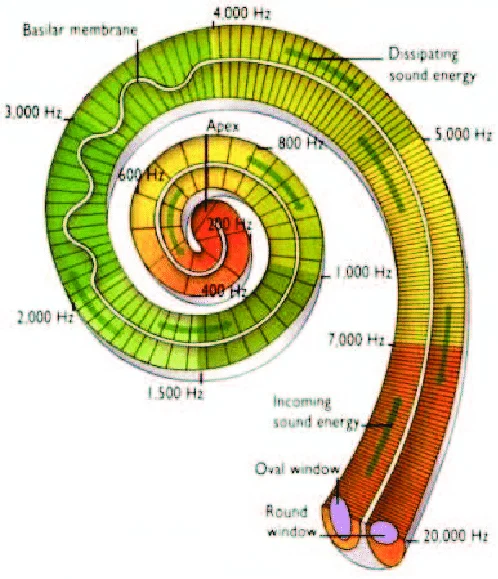
\includegraphics[width=0.38\textwidth]{../assets/figures/ch05-basilar-membrane.png}}
  \caption{نقشهٔ تونوتوپیک حلزون گوش. رأس حلزون (\eng{Apex}) مربوط به فرکانس‌های بم و قاعدهٔ آن (\eng{Base}) نزدیک دریچه‌های بیضی و گرد مربوط به فرکانس‌های زیر است. اعداد روی تصویر فرکانس تقریبی نقاط مختلف را نشان می‌دهند. \textit{(برگرفته از تختهٔ کلاس)}}
  \label{fig:cochlea}
\end{figure}

\subsection{سازمان‌دهی فرکانسی}
\begin{itemize}
  \item \textbf{قاعده یا \eng{Base}}: ناحیهٔ ابتدایی حلزون که صدا نخست به آن می‌رسد؛ به فرکانس‌های \emph{بالا} (زیر) حساس است.
  \item \textbf{رأس یا \eng{Apex}}: انتهای مارپیچ حلزون؛ به فرکانس‌های \emph{پایین} (بم) حساس است.
  \item هر بخش از غشای پایه به یک محدودهٔ فرکانسی معین حساس‌تر است؛ بنابراین توزیع فرکانس‌ها در دستگاه شنوایی تصادفی نیست و یک «نقشه» دارد.
\end{itemize}

\begin{correctionbox}{دقت در خواندن شکل}
نمودار حلزون در شکل \ref{fig:cochlea} ساده‌شده است: عدد نوشته‌شده نزدیک رأس (حدود ۲۰۰ هرتز) حد پایین واقعی شنوایی نیست؛ شنوایی انسان تا حدود ۲۰ هرتز ادامه دارد و ناحیهٔ بسیار کوچک رأس به همین فرکانس‌های خیلی بم مربوط می‌شود. همچنین فاصلهٔ مکانی روی غشای پایه با \emph{فرکانس} رابطهٔ خطی ندارد، بلکه تقریباً با \emph{لگاریتم فرکانس} متناسب است (رابطهٔ تجربی گرین‌وود): نیمهٔ رأسی حلزون به‌تنهایی مربوط به فرکانس‌های زیر حدود $1.5$ تا ۲ کیلوهرتز است و فرکانس‌های بالاتر در نیمهٔ دیگر فشرده شده‌اند. همین فشردگی ریشهٔ فیزیولوژیک بحث مقیاس مل در ادامه است.
\end{correctionbox}

\subsection{تفکیک نابرابر فرکانس‌های بم و زیر}
نتیجهٔ مهم این سازمان‌دهی آن است که ادراک تغییرات فرکانسی \emph{خطی نیست}. دو تغییر زیر را مقایسه کنید:
\[
100 \;\rightarrow\; 200\ \text{\lr{Hz}}
\qquad\text{و}\qquad
5100 \;\rightarrow\; 5200\ \text{\lr{Hz}}.
\]
در هر دو، اختلاف فرکانس ۱۰۰ هرتز است؛ اما تغییر اول برای گوش بسیار چشمگیر و تغییر دوم تقریباً نامحسوس است. یعنی میزان تفاوت ادراکی فقط به \emph{اختلاف عددی} بستگی ندارد، بلکه به \emph{محدودهٔ فرکانسی} بستگی دارد. دو مثال شهودی که در کلاس مطرح شد:
\begin{itemize}
  \item \textbf{صدای موتور}: مؤلفه‌های غالب فرکانس پایین‌اند و تغییر نسبتاً کوچکی در آن‌ها (مثلاً هنگام تغییر دور موتور) به‌سادگی شنیده می‌شود.
  \item \textbf{صدای سوت}: فرکانس بالایی دارد و اگر فرکانسش کمی تغییر کند، تشخیص تفاوت دو صدا دشوارتر است.
\end{itemize}
به بیان کلاس: گوش ما در فرکانس‌های پایین (زیر حدود ۱۰۰۰ هرتز) بسیار دقیق است، اما در فرکانس‌های بالا (بالای حدود ۴۰۰۰ هرتز) تفاوت‌ها را به‌خوبی تشخیص نمی‌دهد.

\begin{correctionbox}{دقت علمی دربارهٔ «تفاضل مهم نیست، نسبت مهم است»}
جمع‌بندی دقیق‌تر این است که توان تفکیک فرکانسی گوش (کوچک‌ترین تفاوت قابل‌تشخیص، \eng{JND}) در فرکانس‌های زیر حدود ۵۰۰ تا ۱۰۰۰ هرتز در حد چند هرتز است و در فرکانس‌های بالاتر تقریباً با خود فرکانس بزرگ می‌شود (یعنی نسبت‌محور است). بنابراین تغییر ۱۰۰ هرتز در ۵ کیلوهرتز برای شنوندهٔ آموزش‌دیده در آزمایشگاه \emph{هنوز قابل‌تشخیص} است؛ نکتهٔ درست این است که برای گوش، آن تغییر بسیار کوچک‌تر از تغییر ۱۰۰ به ۲۰۰ هرتز به‌نظر می‌رسد (در مقیاس ادراکی). این همان چیزی است که مقیاس مل می‌خواهد مدل کند.
\end{correctionbox}

\begin{addedbox}{مقایسهٔ عددی دو تغییر ۱۰۰ هرتزی}
اگر تغییر فرکانس را به‌صورت «نسبت» بسنجیم، تغییر ۱۰۰ به ۲۰۰ هرتز یک اکتاو کامل است (نسبت ۲، یعنی ۱۲۰۰ سنت)، اما تغییر ۵۱۰۰ به ۵۲۰۰ هرتز فقط نسبت $5200/5100\approx 1.0196$ است:
\[
1200\log_2\frac{5200}{5100}\approx 33.6\ \text{سنت}\qquad\text{(حدود \(\tfrac{1}{36}\) اکتاو)}.
\]
در مقیاس مل (بخش بعد) همین دو تغییر به‌ترتیب حدود \textbf{$132.7$} و \textbf{$19.3$} مل‌اند؛ یعنی تغییر اول از نظر ادراکی بیش از ۶ برابر بزرگ‌تر است.
\end{addedbox}

\subsection{پیامد برای طراحی ویژگی}
اگر بخواهیم ویژگی‌هایی متناسب با شنوایی انسان بسازیم، نباید همهٔ بازه‌های فرکانسی را با دقت یکسان نمایش دهیم. می‌خواهیم:
\begin{itemize}
  \item در فرکانس‌های پایین تفکیک بیشتر (بازه‌های باریک) داشته باشیم؛
  \item در فرکانس‌های بالا بازه‌های گسترده‌تری را در یک گروه جمع کنیم؛
  \item ویژگی‌ها را طوری بسازیم که به ساختار ادراک شنیداری نزدیک‌تر باشند.
\end{itemize}
این ایده مبنای مقیاس مل است.

%====================================================================
\section{مرور سه ویژگی \eng{Pitch}، \eng{Formant} و \eng{Intensity} در \eng{Praat}}
%====================================================================

پیش از رفتن به سراغ مل، استاد با نمایش یک سیگنال گفتاری در نرم‌افزار \eng{Praat} سه ویژگی مهم را مرور کرد. در نمایش پیش‌فرض این نرم‌افزار، روی اسپکتروگرام خاکستری، مسیر فرمنت‌ها با نقطه‌های قرمز، مسیر \eng{pitch} با خط آبی و منحنی شدت صوت با خط زرد نشان داده می‌شود.

\begin{itemize}
  \item \term{فرمنت}{Formant}: نواحی تشدید طیفی که در بررسی واکه‌ها اهمیت دارند و با $F_1$، $F_2$ و $F_3$ نشان داده می‌شوند. در جلسات قبل از آن‌ها برای ساخت فضای واکه‌ای استفاده کردیم.
  \item \term{پیچ}{Pitch}: ادراک زیر و بمی صدا که با فرکانس پایه ($F_0$، تناوب سیگنال) ارتباط نزدیک دارد، اما با آن یکی نیست: $F_0$ کمیتی فیزیکی است و \eng{pitch} کمیتی ادراکی.
  \item \term{شدت}{Intensity}: معیاری از «قدرت» کلی صوت در هر لحظه. برخلاف طیف که انرژی هر فرکانس را جداگانه نشان می‌دهد، منحنی \eng{intensity} تغییر شدت کلی را در طول زمان نمایش می‌دهد (فریاد‌زدن شدت زیاد، صحبت آرام شدت کم).
\end{itemize}

\begin{table}[htbp]
\centering
\caption{تمایز کمیت‌های فیزیکی و ادراکی که باید از هم جدا نگه داشته شوند.}
\begin{tabular}{p{4cm}p{4.5cm}p{4cm}}
\toprule
\textbf{کمیت فیزیکی} & \textbf{کمیت ادراکی متناظر} & \textbf{توضیح} \\
\midrule
فرکانس پایه \eng{($F_0$)} & زیر و بمی (\eng{Pitch}) & تناوب موج در برابر احساس زیر/بم \\
شدت (\eng{Intensity}) & بلندی (\eng{Loudness}) & توان فیزیکی در برابر بلندی احساس‌شده \\
فرمنت‌ها / شکل طیف & رنگ صدا (\eng{Timbre}) و کیفیت واکه & تشدیدهای مجرای صوتی \\
\bottomrule
\end{tabular}
\end{table}

زیر و بمی با بلندی یکی نیست: یک فرد می‌تواند با صدای زیر ولی بسیار آرام صحبت کند یا با صدای بم و پرشدت. این دو بُعد باید جداگانه بررسی شوند، و این تمایز میان «شدت فیزیکی» و «بلندی ادراک‌شده» در بخش لگاریتم دوباره مهم می‌شود.

\begin{correctionbox}{محاسبهٔ دقیق شدت صوت}
در کلاس گفته شد که شدت را می‌توان به‌صورت شهودی «تجمیع انرژی مؤلفه‌های فرکانسی در یک لحظه» دید. این شهود درست است، ولی محاسبهٔ دقیق جمع ساده‌ٔ مقدارهای اندازه (\eng{magnitude}) طیف نیست. شدت بر پایهٔ \emph{مربع} دامنه (توان) محاسبه می‌شود و (طبق رابطهٔ پارسوال) جمع مربعات اندازهٔ طیف با میانگین مربع موج در حوزهٔ زمان برابر است. در \eng{Praat} شدت از مربع نمونه‌های سیگنال در یک پنجرهٔ زمانی هموارکننده به دست می‌آید و بر حسب دسی‌بل نسبت به فشار مرجع $2\times10^{-5}$ پاسکال گزارش می‌شود.
\end{correctionbox}

\begin{exambox}{پرسش و پاسخ: چرا خط \eng{pitch} بالاتر از نقطه‌های فرمنت دیده می‌شود؟}
یکی از دانشجویان پرسید چرا در تصویر \eng{Praat} گاهی خط آبی \eng{pitch} بالاتر از نقطه‌های قرمز فرمنت است، در حالی که $F_0$ همواره از $F_1$ پایین‌تر است. پاسخ: این نمودارها با \emph{محورهای مختلف} رسم می‌شوند؛ مقیاس \eng{pitch} در یک سمت تصویر و مقیاس فرمنت‌ها در سمت دیگر نمایش داده می‌شود و بنابراین بالاتر بودن خط روی صفحه دلیلی بر بزرگ‌تر بودن مقدار فرکانسی آن نیست. تنظیمات نمایش \eng{pitch} را نیز می‌توان در \eng{Praat} تغییر داد. چگونگی محاسبهٔ کانتور این ویژگی‌ها در جلسهٔ بعد بیشتر بررسی می‌شود.
\end{exambox}

%====================================================================
\section{کم‌شنوایی فرکانس‌های بالا با افزایش سن}
\label{sec:presbycusis}
%====================================================================

یکی از پیامدهای نقشهٔ تونوتوپیک این است که چون ناحیهٔ قاعدهٔ حلزون به فرکانس‌های بالا مربوط است، آسیب به همین ناحیه موجب کاهش توان شنیدن صداهای زیر می‌شود. کم‌شنوایی فرکانس‌های بالا در سنین بالا بسیار رایج است؛ این پدیده را \term{پیرگوشی}{Presbycusis} می‌نامند. به بیان تختهٔ کلاس: وقتی پایهٔ حلزون تحلیل می‌رود، شنونده برای تفکیک و درک گفتارهای دارای فرکانس زیر باید انرژی و تلاش بیشتری صرف کند.

دلیل مطرح‌شده در کلاس این بود که سلول‌های ناحیهٔ \eng{Base} در «خط مقدم» ضربه‌های مکانیکی‌اند، سریع‌تر کار می‌کنند، خون‌رسانی آسیب‌پذیرتری دارند و دفاع آنتی‌اکسیدانی کمتری دارند؛ به همین دلیل در نقشهٔ تونوتوپیک نخستین جایی هستند که با گذر سن تحلیل می‌روند.

\begin{correctionbox}{دقت علمی دربارهٔ علل پیرگوشی}
الگوی کلی (افت شنوایی تدریجی، دوطرفه و عمدتاً در فرکانس‌های بالا) درست است. ولی علت آن چندعاملی است و نباید به یک توضیح ساده تقلیل یابد: از دست رفتن سلول‌های مویی حلزون، تحلیل رگ‌های نوار عروقی (\eng{stria vascularis})، کاهش نورون‌های عصب شنوایی، استرس اکسایشی، سابقهٔ مواجهه با نویز، عوامل ژنتیکی و داروهای آسیب‌رسان به گوش. یکی از دلایل شایعی که برای حساسیت ناحیهٔ قاعده بیان می‌شود این است که \emph{هر صدایی}، صرف‌نظر از فرکانس، ابتدا از ناحیهٔ قاعده عبور می‌کند و آن ناحیه بیشترین بار مکانیکی و متابولیکی را تحمل می‌کند. توضیح تختهٔ کلاس (مکانیکی، خون‌رسانی، دفاع آنتی‌اکسیدانی) در همین چارچوب قابل‌فهم است؛ با این حال، آن را باید «مجموعه‌ای از سازوکارهای محتمل» دانست نه یک علت قطعی.
\end{correctionbox}

\begin{addedbox}{پیامد عملی برای گفتار}
بسیاری از همخوان‌های بی‌واک مانند \eng{/s/}، \eng{/f/} و \eng{/sh/} انرژی عمده‌شان در فرکانس‌های بالا (چند کیلوهرتز) است؛ به همین دلیل افراد دچار پیرگوشی معمولاً در تفکیک این همخوان‌ها و درک گفتار (به‌ویژه در محیط پرنویز) مشکل بیشتری دارند، هرچند صدا را «بلند» می‌شنوند. این مثالی است از اینکه حساسیت شنوایی نه‌تنها در فرکانس‌های مختلف یکسان نیست، بلکه با سن و شرایط فیزیولوژیک نیز تغییر می‌کند.
\end{addedbox}

%====================================================================
\section{مقیاس مل}
%====================================================================

تا اینجا دیدیم که گوش تفاوت فرکانس‌ها را به‌صورت خطی درک نمی‌کند. برای وارد کردن این ویژگی در پردازش گفتار از \term{مقیاس مل}{Mel Scale} استفاده می‌کنیم.

\begin{definitionbox}{مقیاس مل}
مقیاس مل یک \textbf{نگاشت غیرخطی} از فرکانس فیزیکی (بر حسب هرتز) به یک مقیاس ادراکی (بر حسب مل) است که فرکانس‌های بالا را «فشرده» می‌کند تا فاصله‌های برابر روی این محور تقریباً با تفاوت‌های ادراکی برابر در زیر و بمی متناظر باشند. نام «مل» از واژهٔ \eng{melody} (آهنگ) گرفته شده است.
\end{definitionbox}

\begin{correctionbox}{فرمول مقیاس مل}
مقیاس مل را استیونز، فولکمن و نیومن در سال ۱۹۳۷ از آزمایش‌های قضاوت زیر و بمی شنوندگان معرفی کردند. در پردازش گفتار، رایج‌ترین تقریب تحلیلی آن (که در کلاس به‌صورت عددی بیان نشد) چنین است:
\[
m = 2595\,\log_{10}\!\Big(1+\frac{f}{700}\Big)
\qquad\Longleftrightarrow\qquad
f = 700\big(10^{\,m/2595}-1\big).
\]
نسخهٔ طبیعی‌لگاریتمی آن $m=1127\ln(1+f/700)$ است (هر دو یکی‌اند). نگاشت ۱۰۰۰ هرتز به ۱۰۰۰ مل با همین ثابت‌ها برقرار می‌شود. قراردادهای دیگری (مثلاً نسخهٔ اسلینی: خطی در زیر ۱ کیلوهرتز و لگاریتمی در بالاتر) نیز وجود دارند؛ بنابراین خروجی کتابخانه‌های مختلف ممکن است اندکی با هم تفاوت داشته باشد.
\end{correctionbox}

رفتار این تابع دو بخش دارد: در فرکانس‌های پایین (زیر حدود ۱ کیلوهرتز) تقریباً خطی است و در فرکانس‌های بالاتر شیب آن کاهش می‌یابد (رشد لگاریتمی).

\begin{figure}[htbp]
  \centering
  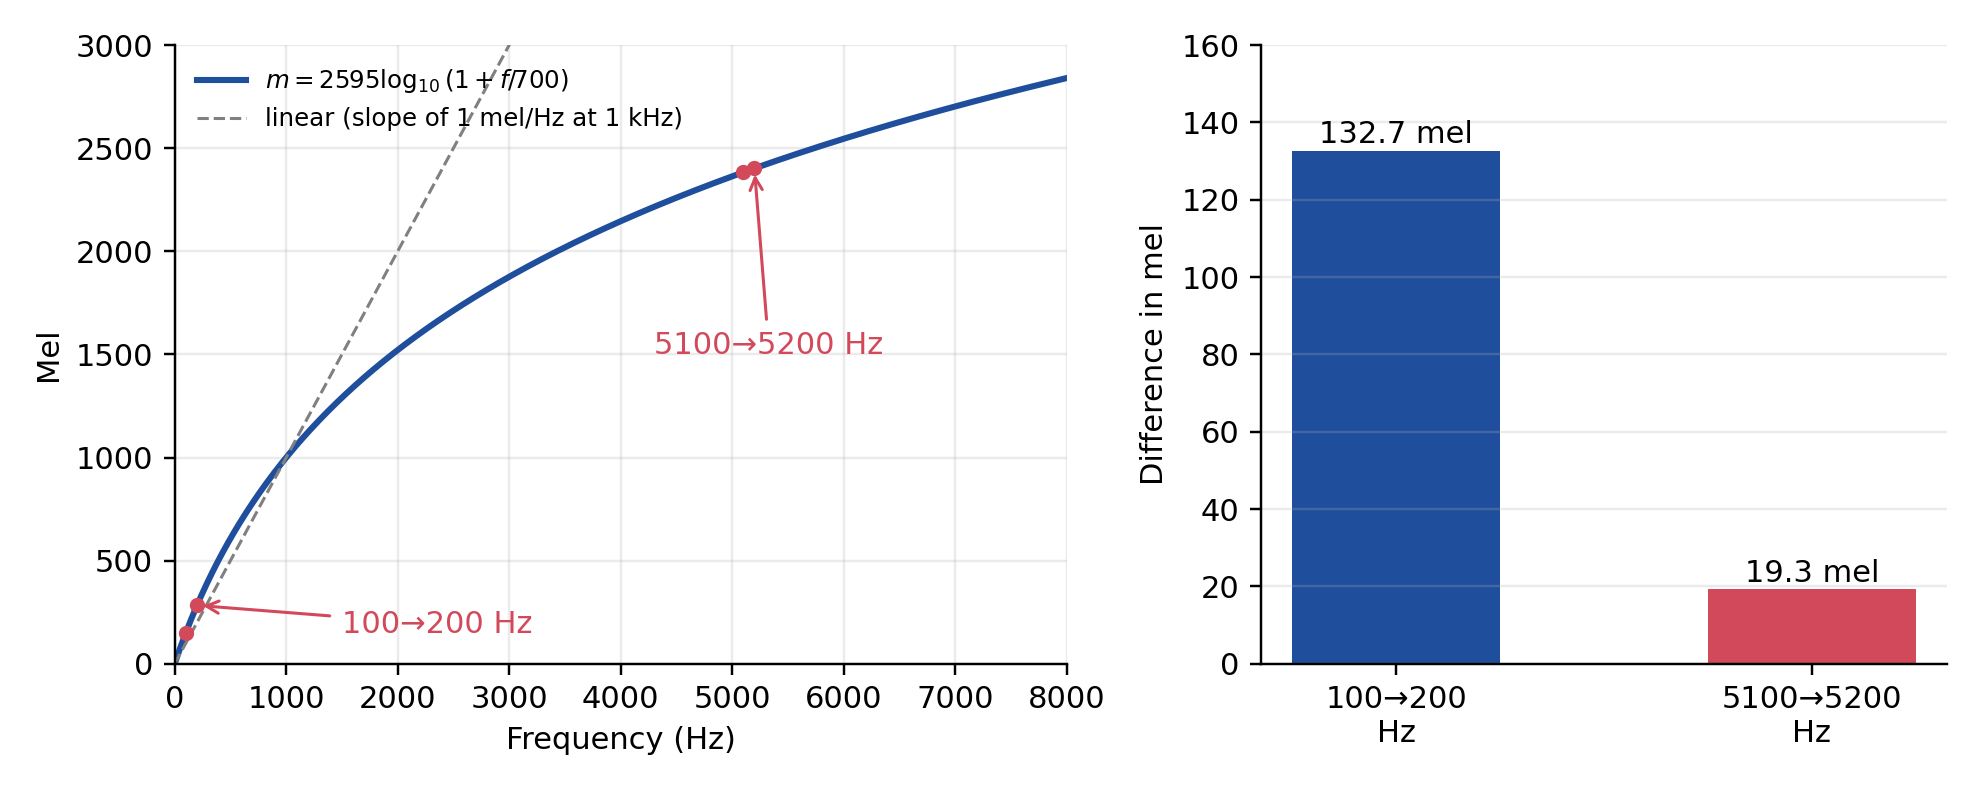
\includegraphics[width=0.95\textwidth]{../assets/figures/ch05-mel-vs-hz.png}
  \caption{چپ: منحنی تبدیل هرتز به مل؛ شیب منحنی در فرکانس‌های بالا کم می‌شود. راست: همان دو تغییر ۱۰۰ هرتزی مثال کلاس در مقیاس مل؛ تغییر ۱۰۰ به ۲۰۰ هرتز بسیار بزرگ‌تر از تغییر ۵۱۰۰ به ۵۲۰۰ هرتز است. (شکل افزوده)}
  \label{fig:melcurve}
\end{figure}

\begin{addedbox}{مثال عددی: تبدیل هرتز به مل}
با فرمول $m=2595\log_{10}(1+f/700)$ برای چند فرکانس:
\begin{center}
\begin{tabular}{rrrrrrrrr}
\toprule
$f$ (هرتز) & 100 & 200 & 500 & 1000 & 2000 & 4000 & 5100 & 8000 \\
\midrule
$m$ (مل) & $150.5$ & $283.2$ & $607.4$ & $1000.0$ & $1521.4$ & $2146.1$ & $2383.1$ & $2840.0$ \\
\bottomrule
\end{tabular}
\end{center}
نمونه:
\[
m(1000)=2595\log_{10}\!\Big(1+\frac{1000}{700}\Big)=2595\times0.3853\approx1000 .
\]
برای عکس مسئله، فرکانس متناظر ۱۵۰۰ مل برابر است با
\[
f=700\,\big(10^{1500/2595}-1\big)=700\times(3.785-1)\approx1949\ \text{هرتز}.
\]
توجه کنید بازهٔ ۰ تا ۸ کیلوهرتز فقط به حدود ۲۸۴۰ مل نگاشت می‌شود و نیمی از این بازهٔ مل (۰ تا ۱۴۲۰ مل) در زیر حدود ۱۷۶۰ هرتز قرار دارد؛ یعنی مقیاس مل به فرکانس‌های پایین «فضای بیشتری» می‌دهد.
\end{addedbox}

\subsection{مسئلهٔ طیف خطی}
فرض کنید طیفی داریم که برای هر فرکانس انرژی (یا اندازهٔ) مشخصی دارد. در نمایش معمول، فرکانس‌ها روی محوری خطی چیده شده‌اند، در حالی که تفکیک گوش خطی نیست. هدف این است که:
\begin{itemize}
  \item اطلاعات فرکانس‌های پایین را با تفکیک بیشتر نگه داریم؛
  \item فرکانس‌های بالا را در بازه‌های پهن‌تر گروه‌بندی کنیم؛
  \item از تعداد زیادی مقدار فرکانسی، مجموعهٔ کوچک‌تری از ویژگی‌های مناسب گفتار بسازیم.
\end{itemize}
ابزار انجام این کار، \textbf{بانک فیلتر مل} است.

%====================================================================
\section{بانک فیلتر مل}
%====================================================================

\term{بانک فیلتر مل}{Mel Filterbank} مجموعه‌ای از فیلترهای مثلثی است که روی محور فرکانس چیده می‌شوند. هر فیلتر یک بازهٔ فرکانسی را پوشش می‌دهد و از اطلاعات آن بازه \emph{یک عدد} استخراج می‌کند: انرژی آن باند.

\begin{figure}[htbp]
  \centering
  \fbox{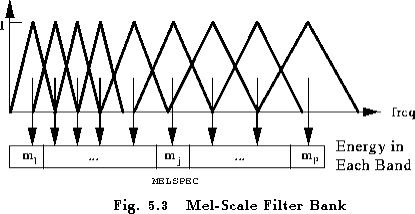
\includegraphics[width=0.55\textwidth]{../assets/figures/ch05-board-filterbank.png}}
  \caption{بانک فیلتر مثلثی مل: فیلترها پشت سر هم و هم‌پوشان چیده شده‌اند و خروجی هر فیلتر انرژی باند متناظر را (\eng{Energy in Each Band}) می‌دهد. با رفتن به فرکانس‌های بالاتر، مثلث‌ها پهن‌تر می‌شوند. \textit{(برگرفته از تختهٔ کلاس)}}
  \label{fig:boardfb}
\end{figure}

\subsection{وزن‌دهی مثلثی}
هر فیلتر سه بخش دارد: ابتدای بازه که وزن نزدیک صفر است، مرکز بازه که وزن به بیشینه (معمولاً ۱) می‌رسد، و انتهای بازه که وزن دوباره به صفر می‌رسد. بنابراین فرکانس‌های نزدیک مرکز فیلتر سهم بیشتری دارند. مقدار طیفی هر فرکانس در وزن متناظر ضرب و حاصل‌ها جمع می‌شوند:
\[
S_m=\sum_{k} H_m[k]\,P[k],
\]
که در آن $P[k]$ طیف توان (یا اندازه) در پایهٔ $k$ام و $H_m[k]$ وزن فیلتر $m$ام است. خروجی هر فیلتر یک عدد است که اطلاعات طیفی بازهٔ زیر پوشش خود را خلاصه می‌کند.

\begin{exambox}{مثال عددی کلاس: خروجی یک فیلتر}
فرض کنید فیلتری سه مؤلفهٔ طیفی با مقدارهای ۴، ۸ و ۶ و وزن‌های $0.5$، ۱ و $0.5$ دریافت کند (اعداد صرفاً آموزشی‌اند). خروجی برابر است با
\[
M_1=(4\times0.5)+(8\times1)+(6\times0.5)=2+8+3=13 .
\]
یعنی به‌جای نگه‌داشتن سه مقدار جداگانه، یک عدد داریم. این کار برای همهٔ فیلترهای بانک تکرار می‌شود.
\end{exambox}

\subsection{چرا فیلترها هم‌پوشان‌اند؟}
فیلترهای مجاور هم‌پوشانی دارند؛ یعنی یک فرکانس ممکن است در محاسبهٔ خروجی دو فیلتر مجاور مشارکت کند. دلیل آن این است که اطلاعات فرکانس‌های نزدیک به مرز دو باند ناگهان حذف یا دچار تغییر پرشی نشود. در طراحی استاندارد، قلهٔ هر مثلث دقیقاً روی نقطهٔ صفر مثلث قبلی و بعدی قرار می‌گیرد؛ در نتیجه مجموع وزن همهٔ فیلترها در هر نقطه (جز دو لبهٔ محور) برابر ۱ است و حساسیت کلی روی محور فرکانس صاف و پیوسته می‌ماند.

مثال تختهٔ کلاس برای فهم ضرورت هم‌پوشانی: فرض کنید مرز دو باند روی ۳۰۰ هرتز باشد و فیلترها مستطیلی و بدون هم‌پوشانی باشند. اگر گوینده فقط ۱ هرتز تغییر کند (مثلاً از ۲۹۹ به ۳۰۱)، آن مؤلفه ناگهان از یک فیلتر خارج و وارد فیلتر دیگر می‌شود و خروجی‌ها پرش می‌کنند. با مثلث‌های هم‌پوشان، همین تغییر کوچک فقط تغییر هموار و کوچکی در خروجی‌ها ایجاد می‌کند.

\subsection{چرا عرض فیلترها یکسان نیست؟}
مهم‌ترین نکتهٔ بانک فیلتر مل: روی محور \emph{خطی} فرکانس، عرض فیلترها یکسان نیست. فیلترها در فرکانس‌های پایین باریک و در فرکانس‌های بالا پهن‌اند (در کلاس: هرچه به فرکانس‌های بالاتر می‌رویم عرض مثلث‌ها، یعنی \eng{Bandwidth}، بیشتر می‌شود و این یعنی دقت در فرکانس‌های بالا کمتر است). دلیل آن است که فیلترها روی \emph{محور مل} یکسان و هم‌فاصله‌اند و وقتی به هرتز برگردانده می‌شوند، در فرکانس‌های بالا پهن می‌شوند. این همان ایدهٔ نقشهٔ تونوتوپیک است.

\begin{figure}[htbp]
  \centering
  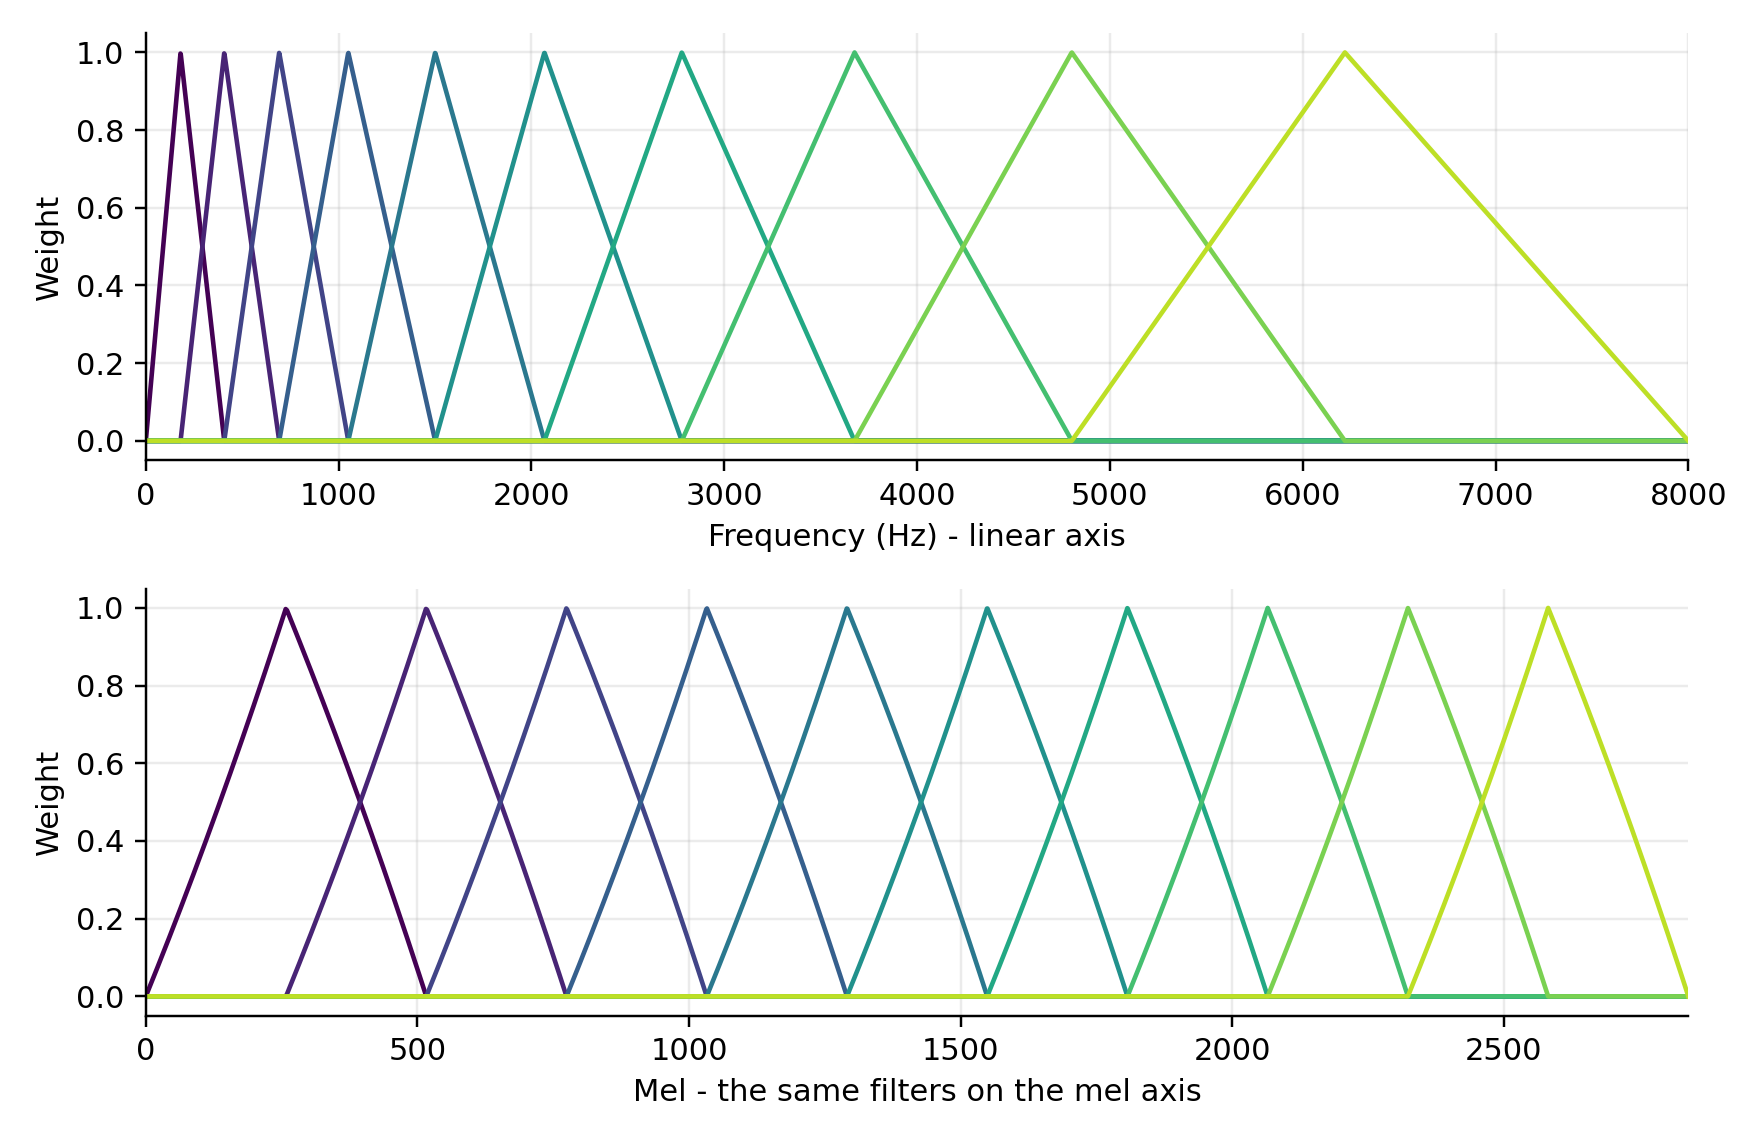
\includegraphics[width=0.9\textwidth]{../assets/figures/ch05-mel-filterbank.png}
  \caption{نمونهٔ یک بانک ده‌فیلتری برای بازهٔ ۰ تا ۸ کیلوهرتز. بالا: روی محور خطی هرتز، فیلترها به‌تدریج پهن می‌شوند. پایین: همان فیلترها روی محور مل، مثلث‌هایی یکسان و هم‌فاصله‌اند. در هر دو نمودار قلهٔ هر فیلتر روی صفر فیلترهای مجاور است. (شکل افزوده)}
  \label{fig:fbplot}
\end{figure}

\begin{addedbox}{ساختن بانک فیلتر: الگوریتم و اعداد}
برای ساخت $M$ فیلتر بین $f_{\min}$ و $f_{\max}$: (۱) هر دو را به مل ببرید؛ (۲) $M+2$ نقطهٔ هم‌فاصله روی محور مل بگذارید؛ (۳) نقاط را به هرتز برگردانید؛ (۴) فیلتر $m$ با لبه‌های $f_{m-1}$ و $f_{m+1}$ و قلهٔ $f_m$ تعریف می‌شود:
\[
H_m[k]=\begin{cases}
0 & f[k]<f_{m-1}\\[2pt]
\dfrac{f[k]-f_{m-1}}{f_m-f_{m-1}} & f_{m-1}\le f[k]\le f_m\\[8pt]
\dfrac{f_{m+1}-f[k]}{f_{m+1}-f_m} & f_m\le f[k]\le f_{m+1}\\[8pt]
0 & f[k]>f_{m+1}.
\end{cases}
\]
مثال: برای $M=40$ و بازهٔ ۰ تا ۸۰۰۰ هرتز (۲۸۴۰ مل)، فاصلهٔ نقاط $2840/41\approx69.3$ مل است. فیلتر اول لبه‌های ۰، ۴۴ و ۹۲ هرتز (عرض $\approx$ ۹۲ هرتز) و فیلتر چهلم لبه‌های حدود ۶۹۹۴، ۷۴۸۱ و ۸۰۰۰ هرتز (عرض $\approx$ ۱۰۰۰ هرتز) دارد؛ یعنی عرض فیلتر آخر بیش از ۱۰ برابر فیلتر اول است. با تبدیل فوریهٔ ۵۱۲ نقطه‌ای در \eng{16 kHz} (فاصلهٔ پایه‌ها $31.25$ هرتز) فیلتر اول فقط روی ۲ ــ ۳ پایه و فیلتر آخر روی حدود ۳۲ پایه سوار است.
\end{addedbox}

\subsection{تعداد فیلترها}
در کلاس گفته شد که در بسیاری از پیاده‌سازی‌ها حدود ۴۰ فیلتر مل به کار می‌رود؛ خروجی هر فریم یک بردار ۴۰‌تایی است:
\[
\mathbf{M}=[M_1,M_2,\ldots,M_{40}].
\]
استاد تأکید کرد که عدد ۴۰ یک مقدار تجربی و متداول است نه ثابت اجباری؛ بسته به مسئله می‌توان آن را تغییر داد.

\begin{addedbox}{مقادیر رایج}
تعداد فیلتر در ابزارهای مختلف متفاوت است: در \eng{HTK} برای گفتار \eng{16 kHz} معمولاً ۲۶ فیلتر، در \eng{Kaldi} حدود ۲۳ فیلتر (برای \eng{MFCC})، و در مدل‌های عصبی (log-mel) رایج است ۴۰، ۸۰ یا ۱۲۸ فیلتر به کار رود (مثلاً \eng{Whisper} از ۸۰ و نسخهٔ جدیدتر آن از ۱۲۸ کانال مل استفاده می‌کند).
\end{addedbox}

\begin{correctionbox}{طیف توان یا اندازه؟}
در کلاس گفته شد که اندازهٔ (\eng{magnitude}) خروجی فوریه در مثلث‌ها ضرب می‌شود. هر دو روش در عمل دیده می‌شوند، اما در تعریف استاندارد \eng{MFCC} فیلترها روی \emph{طیف توان} (مربع اندازه، انرژی) اعمال می‌شوند؛ چون عنوان «انرژی هر باند» مدنظر است. اگر اندازه استفاده شود، ضرایب نهایی با مقیاس متفاوتی به دست می‌آیند.
\end{correctionbox}

\begin{exambox}{پرسش و پاسخ: آیا با ادغام فرکانس‌ها اطلاعات را از دست نمی‌دهیم؟}
چرا، عمداً اطلاعات را \emph{خلاصه} می‌کنیم. هدف نگه‌داشتن طیف اصلی بدون تغییر نیست؛ هدف ساختن نمایشی مناسب‌تر برای گفتار است. تفکیک ریز فرکانس‌های بالا از دید ادراک شنوایی اهمیت کمتری دارد، پس می‌توان بازه‌های بزرگ‌تری را در آن ناحیه ادغام کرد، و هم‌پوشانی فیلترها از حذف ناگهانی اطلاعات مرزی جلوگیری می‌کند. این همان ایدهٔ «فشرده‌سازی مطابق ادراک» است.
\end{exambox}

%====================================================================
\section{ادراک غیرخطی بلندی صدا و لگاریتم}
%====================================================================

گوش علاوه بر غیرخطی بودن در \emph{فرکانس}، در \emph{شدت} نیز غیرخطی است: بلندی ادراک‌شده با افزایش خطی شدت فیزیکی صوت به‌صورت خطی تغییر نمی‌کند. اگر شدت فیزیکی صدای یک گوینده ۱۰۰ برابر شود، احساس نمی‌کنیم صدا ۱۰۰ برابر بلندتر شده است، بلکه فقط چند برابر. این ویژگی (که به‌صورت محافظت از گوش و گسترهٔ پویای وسیع آن نیز تعبیر می‌شود) به سیستم شنوایی اجازه می‌دهد با گسترهٔ بسیار وسیعی از شدت‌ها کار کند.

\subsection{راه‌حل: لگاریتم}
برای وارد کردن این ویژگی، از خروجی هر فیلتر مل لگاریتم می‌گیریم:
\[
L_i=\log(M_i),\qquad \mathbf{L}=[\log M_1,\log M_2,\ldots,\log M_{40}].
\]
لگاریتم تغییرات بسیار بزرگ را فشرده می‌کند:
\[
\log_{10}(10)=1,\quad \log_{10}(100)=2,\quad \log_{10}(1000)=3 .
\]
ورودی از ۱۰ تا ۱۰۰۰ (۱۰۰ برابر) رشد کرده، ولی خروجی فقط از ۱ به ۳ رسیده است. در کلاس تأکید شد که در این مرحله فقط روی \emph{شدت} لگاریتم گرفته می‌شود و به زیر و بمی کاری نداریم.

\begin{correctionbox}{لگاریتم، تقریبی از بلندی؛ نه خود بلندی}
لگاریتم یک مدل ساده و مناسب از فشردگی بلندی است، نه رابطهٔ دقیق آن. آزمایش‌های روان‌فیزیکی (قانون توانی استیونز) نشان می‌دهند بلندی تقریباً با $I^{0.3}$ متناسب است: به‌ازای هر ۱۰ دسی‌بل افزایش تراز، بلندی حدود دو برابر می‌شود. پس اگر شدت ۱۰۰ برابر (۲۰ دسی‌بل) شود، بلندی حدود $100^{0.3}\approx4$ برابر می‌شود، نه ۱۰۰ برابر. لگاریتم و توان $0.3$ هر دو منحنی‌هایی با شیب کاهنده‌اند و در عمل لگاریتم مناسب و ساده‌تر است. به‌علاوه، گسترهٔ پویای گوش از آستانهٔ شنوایی تا آستانهٔ درد حدود $10^{12}$ برابر توان (۱۲۰ دسی‌بل) است؛ مقیاس دسی‌بل خود یک مقیاس لگاریتمی است.
\end{correctionbox}

\begin{figure}[htbp]
  \centering
  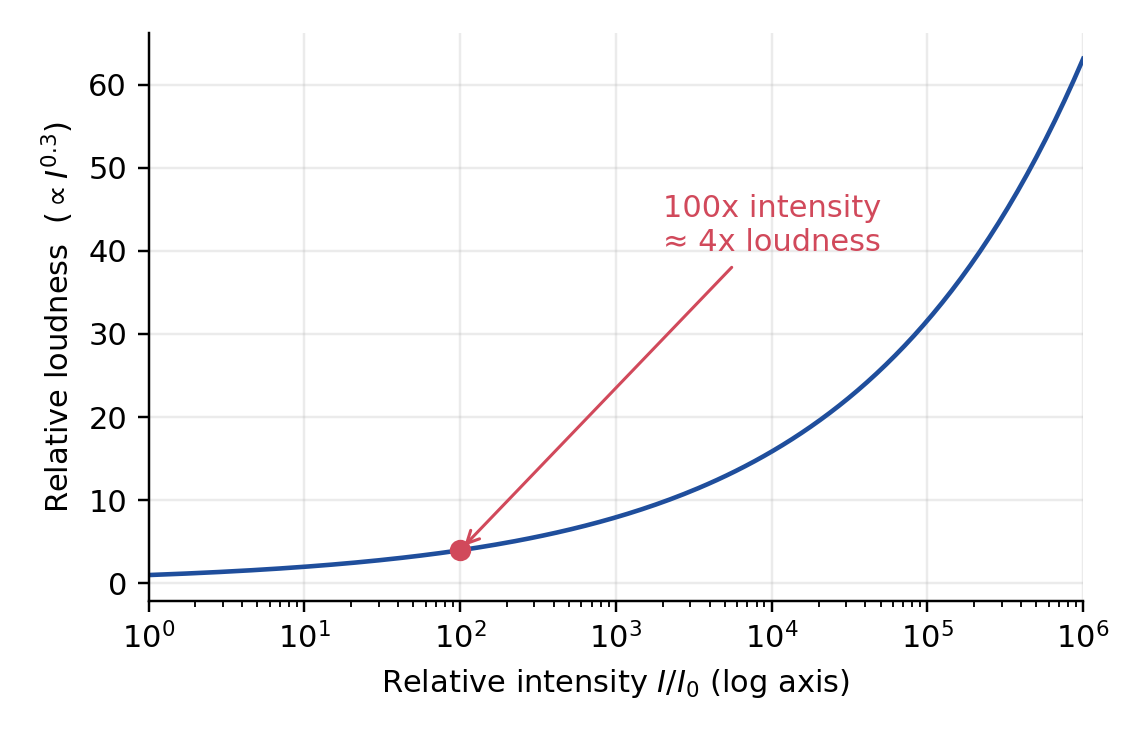
\includegraphics[width=0.6\textwidth]{../assets/figures/ch05-loudness-log.png}
  \caption{بلندی نسبی ($\propto I^{0.3}$) در برابر شدت نسبی. با ۱۰۰ برابر شدن شدت فیزیکی، بلندی حدود ۴ برابر می‌شود؛ منحنی روی محور لگاریتمی شدت رسم شده است. (شکل افزوده)}
\end{figure}

\begin{warningbox}{لگاریتم صفر!}
اگر خروجی یک فیلتر دقیقاً صفر باشد (مثلاً در سکوت دیجیتال)، $\log 0=-\infty$ می‌شود. در پیاده‌سازی عملی یک مقدار کوچک $\varepsilon$ (مثلاً $10^{-10}$) به انرژی اضافه یا کف مناسبی برای آن در نظر گرفته می‌شود: $L_i=\log(M_i+\varepsilon)$.
\end{warningbox}

\begin{addedbox}{مزیت‌های دیگر لگاریتم}
افزون بر ادراک، لگاریتم یک مزیت پردازشی هم دارد: ضرب را به جمع تبدیل می‌کند. اگر سیگنال $x$ از کانالی (میکروفون، اتاق) با پاسخ فرکانسی $h$ عبور کند، در حوزهٔ طیف $|Y|=|X||H|$ و در حوزهٔ لگاریتم $\log|Y|=\log|X|+\log|H|$؛ یعنی اثر کانال به‌صورت یک مقدار ثابت جمع‌شونده در می‌آید و با تکنیک‌هایی مانند حذف میانگین کپسترال (\eng{CMN}) قابل حذف است.
\end{addedbox}

\subsection{جمع‌بندی دو مرحلهٔ نخست}
\begin{table}[htbp]
\centering
\caption{دو ادراک غیرخطی شنوایی و راه‌حل‌های متناظر آن‌ها در \eng{MFCC}.}
\begin{tabular}{p{5.5cm}p{6cm}}
\toprule
\textbf{مسئله} & \textbf{راه‌حل} \\
\midrule
ادراک غیرخطی تفاوت فرکانس‌ها & مقیاس مل و بانک فیلتر مل \\
ادراک غیرخطی تغییرات شدت صوت & تبدیل لگاریتمی \\
\bottomrule
\end{tabular}
\end{table}

%====================================================================
\section{افزونگی ویژگی‌ها و تبدیل کسینوسی گسسته}
%====================================================================

پس از بانک فیلتر مل و لگاریتم، برای هر فریم گفتار ۴۰ عدد داریم. اما این ۴۰ عدد کاملاً مستقل نیستند: فیلترهای مجاور هم‌پوشان‌اند و اطلاعات طیفی مجاور را می‌بینند، پس خروجی بسیاری از آن‌ها شباهت و هم‌بستگی زیاد (\eng{Correlation}) دارد؛ اطلاعات بخشی از آن‌ها تکراری یا کم‌اهمیت‌تر است. می‌خواهیم تعداد ویژگی‌ها را کم کنیم، به شکلی که بخش مهم اطلاعات حفظ شود.

\subsection{یک تبدیل دیگر روی دنباله}
ایدهٔ مرحلهٔ بعد این است که روی همین دنبالهٔ ۴۰تایی یک تبدیل دیگر اعمال کنیم. در تختهٔ کلاس این مرحله چنین توضیح داده شد: «یک فوریهٔ مجدد (\eng{DCT}) به این ۴۰ عدد می‌زنیم تا عصارهٔ آن‌ها را بکشیم». از خروجی این تبدیل، ۱۲ یا ۱۳ ضریب اول نگه داشته می‌شوند و همین‌ها \eng{MFCC} نام دارند. استاد این مرحله را به‌صورت شهودی «انجام یک تبدیل فوریهٔ دیگر» توضیح داد و گفت این ۱۲ــ۱۳ عدد «خالص‌ترین شناسهٔ شکل دهان و واج‌های گفتار» هستند و حجم داده را هم برای مدل‌ها بسیار کم می‌کنند.

تبدیل کسینوسی گسسته (\term{تبدیل کسینوسی گسسته}{Discrete Cosine Transform, DCT}) دنبالهٔ ورودی را به ترکیبی از کسینوس‌هایی با فرکانس‌های رو به افزایش تجزیه می‌کند. برای $M$ مقدار لگاریتمی $L_1,\ldots,L_M$:
\[
c_n=\sum_{m=1}^{M} L_m\cos\!\Big(\frac{\pi n\,(m-\tfrac12)}{M}\Big),\qquad n=0,1,\ldots,12 .
\]
اینجا دنبالهٔ $L_m$ را مانند یک «سیگنال» می‌بینیم که متغیر مستقل آن به‌جای زمان، \emph{شمارهٔ فیلتر (فرکانس)} است. ضرایب پایین‌تر ($n$ کوچک) تغییرات کند و کلی شکل طیف (پوش طیف) را توصیف می‌کنند و ضرایب بالاتر تغییرات سریع و ریز را.

\begin{correctionbox}{چرا DCT هم‌بستگی را کم می‌کند؟}
دلیل دقیق: لگاریتم انرژی فیلترهای مجاور به‌سبب هم‌پوشانی و هموار بودن پوش طیف بسیار هم‌بسته است. پایه‌های \eng{DCT} (کسینوس‌ها) متعامدند و برای دنباله‌های هموار و به‌شدت هم‌بسته (مانند فرایند مارکوف مرتبهٔ اول با هم‌بستگی بالا) تقریب بسیار خوبی از تبدیل \term{کارونن‌لوو}{Karhunen-Loève Transform} (همان \eng{PCA}) هستند؛ یعنی بیشترِ انرژی در چند ضریب نخست جمع می‌شود و ضرایب خروجی تقریباً ناهم‌بسته‌اند. این ناهم‌بستگی در تاریخ تشخیص گفتار مهم بود، چون مدل‌های \eng{GMM} با ماتریس کوواریانس قطری را روی \eng{MFCC} امکان‌پذیر می‌ساخت.
\end{correctionbox}

\begin{addedbox}{مثال عددی: فشردگی انرژی با DCT}
دنبالهٔ هموار شش‌تایی زیر (شبیه دنبالهٔ نوشته‌شده روی تخته) را در نظر بگیرید که دو سطح تقریباً ثابت دارد:
\[\mathbf{x}=[5,\,5.2,\,4.9,\,8,\,8.1,\,7.9].\]
\eng{DCT} متعامد آن (نسخهٔ \eng{DCT-II} با نرمال‌سازی متعامد) برابر است با
\[
\mathbf{c}\approx[\,15.96,\;-3.26,\;0.00,\;1.27,\;-0.23,\;-0.98\,].
\]
مجموع مربعات هر دو دنباله برابر $268.07$ است (پایستگی انرژی)، ولی دو ضریب اول به‌تنهایی حدود \textbf{۹۹٪} انرژی را دارند. اگر فقط این دو ضریب را نگه داریم و دنباله را بازسازی کنیم، به دنبالهٔ
\[\hat{\mathbf{x}}\approx[4.7,\,5.2,\,6.0,\,7.0,\,7.9,\,8.3]\]
می‌رسیم که شکل کلی (پایین در ابتدا، بالا در انتها) را حفظ کرده است. این دقیقاً منطق نگه‌داشتن ۱۲ ــ ۱۳ ضریب اول از ۴۰ مقدار است.
\end{addedbox}

\subsection{چرا ۱۲ یا ۱۳ ضریب؟}
دلیل انتخاب این تعداد تجربی است؛ در کاربردهای متداول گفتار دیده شده که چند ضریب اول اطلاعات مفید کافی را دارند. این به معنای بهینه بودن ۱۲ یا ۱۳ در همهٔ مسائل نیست؛ تعداد فیلترها (حدود ۴۰) و تعداد ضرایب (۱۲ یا ۱۳؛ ممکن است ۵ یا بیشتر هم امتحان شود) هر دو \term{ابرپارامتر}{Hyperparameter}اند و باید بر اساس عملکرد سیستم تنظیم شوند.

\begin{figure}[htbp]
  \centering
  \begin{tikzpicture}[rtl, node distance=1.2cm, box/.style={draw, rounded corners, minimum height=1cm, minimum width=3.2cm, align=center, fill=blue!6}]
    \node[box] (a) {\RL{انرژی‌های لگاریتمی مل}\\\lr{40 values}};
    \node[box, left=1.8cm of a, fill=orange!15] (b) {\lr{DCT}};
    \node[box, left=1.8cm of b, fill=green!12] (c) {\RL{ضرایب \lr{MFCC}}\\\lr{12--13 values}};
    \draw[-{Latex}] (a) -- (b);
    \draw[-{Latex}] (b) -- (c);
  \end{tikzpicture}
  \caption{کاهش ابعاد از ۴۰ مقدار به ۱۳ ضریب (حدود $32.5$٪ ابعاد اولیه). (شکل افزوده)}
\end{figure}

\begin{exambox}{پرسش و پاسخ: آیا انتخاب ۱۲ یا ۱۳ ضریب اثبات ریاضی دارد؟}
خیر؛ این انتخاب تجربی است. تعداد ضرایب یک ابرپارامتر است و می‌توان آن را بر اساس عملکرد سیستم در مسئلهٔ موردنظر انتخاب کرد.
\end{exambox}

%====================================================================
\section{کپستروم و روایت تاریخی تحلیل کپسترال}
%====================================================================

\subsection{واژهٔ «کپستروم»}
واژهٔ \term{کپستروم}{Cepstrum} از جابه‌جایی چهار حرف نخست واژهٔ \eng{Spectrum} ساخته شده است. مفهوم آن در کلاس چنین بیان شد: «از یک طیف (اسپکتروم) یک طیف دیگر گرفته شد». بر همین قیاس، محور مستقل کپستروم \term{کوفرنسی}{Quefrency} (از \eng{Frequency}) نام دارد و واحد آن از جنس زمان است.

\subsection{روایت تاریخی}
استاد برای توضیح ایدهٔ تبدیل مجدد اطلاعات طیفی به روایتی از دوران جنگ سرد اشاره کرد: برای ایالات متحده مسئلهٔ مهم این بود که از روی امواج ثبت‌شده تشخیص دهد یک رویداد زلزله بوده یا آزمایش هستهٔ شوروی. هر دو امواج لرزه‌ای ایجاد می‌کنند، اما ویژگی‌های آن‌ها یکسان نیست. در توضیح کلاس، انفجار منبعی متمرکزتر دارد، در حالی که زلزله حاصل فرایندهای گسترده‌تری است، و اعمال تبدیل دوم روی اطلاعات طیفی الگوهایی را آشکار می‌کند که در طیف اولیه به‌آسانی قابل‌استفاده نبود. نکتهٔ اصلی برای ما این است: گاهی با تبدیل‌کردن دوبارهٔ یک نمایش طیفی، اطلاعاتی آشکار می‌شود که در نمایش اولیه دیده نمی‌شود.

\begin{correctionbox}{دقت تاریخی (تأیید روایت)}
اصل روایت درست است و در منابع تاریخ پردازش سیگنال هم آمده است. مفهوم کپستروم را \eng{Bogert}، \eng{Healy} و \eng{Tukey} در مقاله‌ای با عنوان
\begin{latin}
\noindent\textit{``The Quefrency Alanysis of Time Series for Echoes: Cepstrum, Pseudo-Autocovariance, Cross-Cepstrum and Saphe Cracking''}
\end{latin}
در سال ۱۹۶۳ معرفی کردند (مجموعه‌مقالات سمپوزیوم تحلیل سری‌های زمانی، ویراستار \eng{M. Rosenblatt}). موضوع آن تشخیص \emph{پژواک} (\eng{echo}) در رکوردهای لرزه‌نگاری بود، و انگیزهٔ این پژوهش‌ها با تفکیک زلزله از انفجار و نظارت بر آزمایش‌های هسته‌ای مرتبط دانسته می‌شود. نکتهٔ مهم برای دقت: این قیاس به‌معنی استفادهٔ مستقیم از \eng{MFCC} در لرزه‌شناسی نبود؛ \eng{MFCC} بعدها (۱۹۸۰) توسط \eng{Davis} و \eng{Mermelstein} برای تشخیص گفتار معرفی شد. این روایت در جزئیات (مثلاً «منظم‌تر بودن الگوی منبع متمرکز») بازگویی ساده‌شده است.
\end{correctionbox}

\begin{addedbox}{واژه‌های بازی‌گونهٔ تحلیل کپسترال}
نویسندگان آن مقاله (بوگرت، هیلی و توکی) بازی با حروف را برای مفاهیم دیگر نیز ادامه دادند:
\begin{center}
\begin{latin}
\begin{tabular}{lcl}
spectrum & $\rightarrow$ & cepstrum \\
frequency & $\rightarrow$ & quefrency \\
analysis & $\rightarrow$ & alanysis \\
phase & $\rightarrow$ & saphe \\
filtering & $\rightarrow$ & liftering \\
harmonic & $\rightarrow$ & rahmonic \\
\end{tabular}
\end{latin}
\end{center}
از میان این‌ها هنوز \eng{cepstrum}، \eng{quefrency} و \eng{lifter/liftering} در پردازش گفتار به کار می‌رود.
\end{addedbox}

\subsection{کپستروم چه می‌کند؟ شهود پژواک و هارمونیک}
تعریف کپستروم حقیقی:
\[
c[n]=\mathrm{IDFT}\Big\{\log\big|\mathrm{DFT}\{x[n]\}\big|\Big\}.
\]
شهود: اگر یک سیگنال پژواک داشته باشد، لگاریتم طیف آن یک «موج‌دار» تناوبی می‌شود و تبدیل دوم این تناوب را به یک قلهٔ تیز تبدیل می‌کند که جایش تأخیر پژواک را نشان می‌دهد. دقیقاً همین رخداد در گفتار واک‌دار روی می‌دهد: هارمونیک‌های $F_0$ در لگاریتم طیف مانند موج‌هایی با فاصلهٔ $F_0$ دیده می‌شوند و در کپستروم قله‌ای در کوفرنسی $1/F_0$ ایجاد می‌کنند، در حالی که پوش طیف (اثر مجرای صوتی و فرمنت‌ها) که کند تغییر می‌کند در کوفرنسی‌های پایین می‌ماند. به این ترتیب منبع (تارهای صوتی) و فیلتر (مجرا) از هم جدا می‌شوند.

\begin{figure}[htbp]
  \centering
  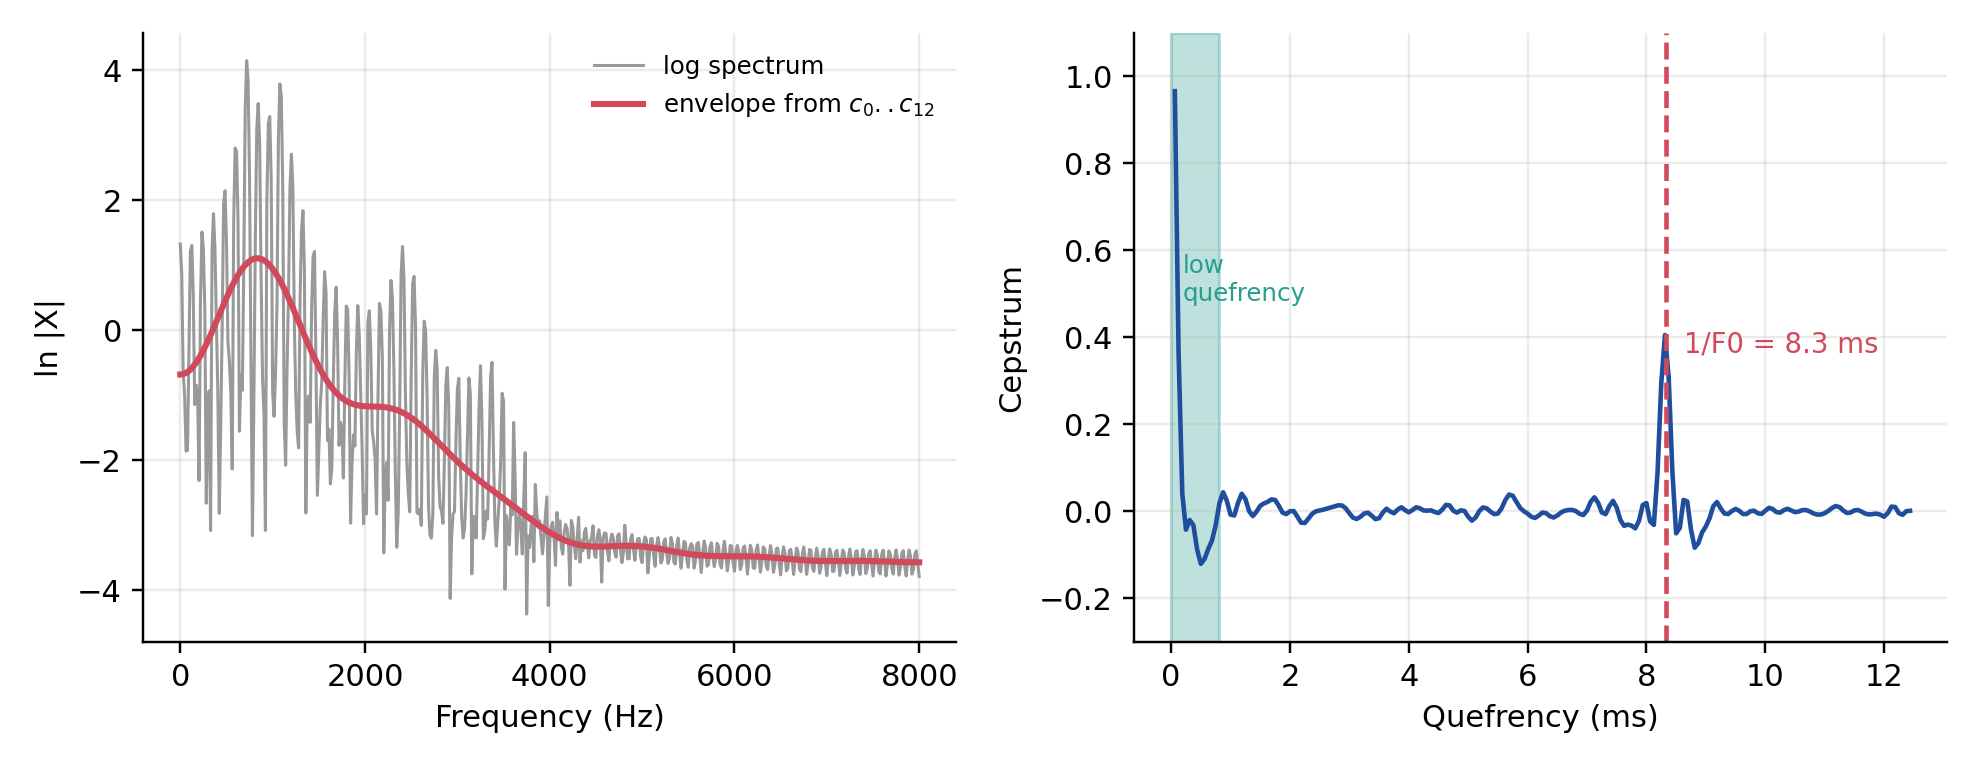
\includegraphics[width=0.95\textwidth]{../assets/figures/ch05-cepstrum.png}
  \caption{کپستروم یک واکهٔ مصنوعی با $F_0=120$ هرتز و فرمنت‌های حدود ۷۳۰، ۱۰۹۰ و ۲۴۴۰ هرتز. چپ: لگاریتم طیف (هارمونیک‌های ریز) و پوش حاصل از ۱۳ ضریب نخست کپستروم. راست: کپستروم با قلهٔ کوفرنسی $1/F_0$ (حدود \eng{8.3 ms}) و ناحیهٔ کوفرنسی پایین مربوط به پوش طیف. (شکل افزوده)}
  \label{fig:cepstrum}
\end{figure}

\begin{correctionbox}{کپستروم کلاسیک و DCT در MFCC یکسان نیستند}
\eng{DCT} در \eng{MFCC} نسخه‌ای از همان ایدهٔ کپستروم است، نه دقیقاً همان عمل: در کپستروم کلاسیک از لگاریتم \emph{طیف کامل} با \eng{IDFT} تبدیل می‌گیریم، اما در \eng{MFCC} ابتدا طیف را روی محور مل و با بانک فیلتر فشرده می‌کنیم، سپس لگاریتم می‌گیریم و از \eng{DCT} استفاده می‌کنیم. (چون لگاریتم طیف توان حقیقی و متقارن است، \eng{IDFT} آن عملاً به یک تبدیل کسینوسی تبدیل می‌شود و \eng{DCT} همین کار را روی دنبالهٔ کوتاه‌تر مل انجام می‌دهد.) با نگه‌داشتن فقط ضرایب اول، عملاً پوش طیف ــ و نه جزئیات ریز هارمونیک‌ها ــ حفظ می‌شود؛ برای همین \eng{MFCC} بیشتر شکل مجرای صوتی (واج) را کد می‌کند و کمتر به $F_0$ حساس است.
\end{correctionbox}

\begin{exambox}{دنبالهٔ مثال تخته}
روی تخته دنبالهٔ
\[[5,\,5.2,\,4.9,\,8,\,8.1,\,7.9,\ldots]\]
نوشته شد؛ منظور مثالی از یک «دنبالهٔ عددی» است که می‌توان آن را مانند یک سیگنال دید و روی آن تبدیل گرفت (مثلاً همین ۴۰ مقدار لگاریتمی مل). اینکه چنین دنبالهٔ هموار بیشتر انرژی‌اش در ضرایب اول جمع می‌شود در مثال عددی بالا دیده شد.
\end{exambox}

%====================================================================
\section{مسیر کامل استخراج MFCC}
%====================================================================

در کلاس مسیر مفهومی چنین بود: سیگنال گفتار $\leftarrow$ تبدیل فوریه (طیف) $\leftarrow$ بانک فیلتر مل $\leftarrow$ لگاریتم $\leftarrow$ \eng{DCT} $\leftarrow$ انتخاب ضرایب اول. در پیاده‌سازی واقعی، چند مرحلهٔ پیش‌پردازش نیز (که در جلسهٔ اسپکتروگرام با پنجره‌های زمانی آشنا شدیم) به ابتدا و انتهای این زنجیره افزوده می‌شود. شکل زیر مسیر کامل و استاندارد را نشان می‌دهد.

\begin{figure}[htbp]
  \centering
  \begin{tikzpicture}[rtl, node distance=0.5cm, blk/.style={draw, rounded corners, minimum width=4.3cm, minimum height=0.75cm, align=center, fill=blue!7, font=\small}, note/.style={font=\footnotesize, text width=5.8cm, align=right}]
    \node[blk, fill=gray!15] (n0) {\RL{سیگنال گفتار (\lr{Waveform})}};
    \node[blk, below=of n0] (n1) {\lr{Pre-emphasis}};
    \node[blk, below=of n1] (n2) {\lr{Framing (25 ms / hop 10 ms)}};
    \node[blk, below=of n2] (n3) {\lr{Windowing (Hamming)}};
    \node[blk, below=of n3] (n4) {\lr{FFT} $\rightarrow$ \lr{Power spectrum}};
    \node[blk, below=of n4, fill=orange!15] (n5) {\lr{Mel Filterbank (40 filters)}};
    \node[blk, below=of n5, fill=orange!15] (n6) {\lr{Log}};
    \node[blk, below=of n6, fill=orange!15] (n7) {\lr{DCT}};
    \node[blk, below=of n7, fill=green!12] (n8) {\lr{MFCC} $c_1\ldots c_{12}$ + \lr{energy}};
    \node[blk, below=of n8, fill=green!12] (n9) {\lr{$\Delta$, $\Delta\Delta$ $\Rightarrow$ 39 features/frame}};
    \foreach \a/\b in {0/1,1/2,2/3,3/4,4/5,5/6,6/7,7/8,8/9} \draw[-{Latex}] (n\a) -- (n\b);
    \node[note, left=0.6cm of n1] {\RL{تقویت فرکانس‌های بالا}};
    \node[note, left=0.6cm of n2] {\RL{هر فریم ۴۰۰ نمونه در \lr{16 kHz}}};
    \node[note, left=0.6cm of n3] {\RL{کاهش نشتی طیفی لبه‌های فریم}};
    \node[note, left=0.6cm of n4] {\lr{512-point FFT $\rightarrow$ 257 bins}};
    \node[note, left=0.6cm of n5] {\RL{بخش ادراکی ۱: مقیاس مل}};
    \node[note, left=0.6cm of n6] {\RL{بخش ادراکی ۲: ادراک لگاریتمی بلندی}};
    \node[note, left=0.6cm of n7] {\RL{حذف هم‌بستگی و فشرده‌سازی}};
    \node[note, left=0.6cm of n9] {\RL{ویژگی‌های پویا (سرعت و شتاب)}};
  \end{tikzpicture}
  \caption{نمودار بلوکی استخراج \eng{MFCC} از سیگنال گفتار تا بردار ویژگی هر فریم. بلوک‌های نارنجی بخش‌هایی هستند که در این جلسه تدریس شد. (شکل افزوده)}
  \label{fig:mfccpipe}
\end{figure}

\subsection{مراحل به‌تفصیل}
\begin{enumerate}
  \item \textbf{پیش‌تأکید (\eng{Pre-emphasis})}: یک فیلتر بالاگذر ساده $y[n]=x[n]-\alpha\,x[n-1]$ با $\alpha\approx0.95\text{--}0.97$ که شیب نزولی طیف گفتار (انرژی کمتر در فرکانس‌های بالا) را جبران می‌کند.
  \item \textbf{فریم‌بندی (\eng{Framing})}: گفتار شبه‌ایستاست؛ پس سیگنال به فریم‌های کوتاه حدود ۲۵ میلی‌ثانیه (۴۰۰ نمونه در \eng{16 kHz}) با گام (\eng{hop}) ۱۰ میلی‌ثانیه (۱۶۰ نمونه) بریده می‌شود، یعنی فریم‌ها ۱۵ میلی‌ثانیه هم‌پوشانی دارند.
  \item \textbf{پنجره‌گذاری (\eng{Windowing})}: ضرب هر فریم در پنجرهٔ همینگ $w[n]=0.54-0.46\cos\!\big(\tfrac{2\pi n}{N-1}\big)$ برای کاهش نشتی طیفی ناشی از بریدگی ناگهانی لبه‌ها.
  \item \textbf{تبدیل فوریه و طیف توان}: \eng{FFT} (معمولاً با ۵۱۲ نقطه با صفر‌گذاری) و $P[k]=|X[k]|^2/N$.
  \item \textbf{بانک فیلتر مل}: ۴۰ (یا ۲۶ و مانند آن) فیلتر مثلثی هم‌پوشان.
  \item \textbf{لگاریتم} انرژی هر فیلتر.
  \item \textbf{\eng{DCT}} و نگه‌داشتن ضرایب $c_1,\ldots,c_{12}$ و افزودن یک ویژگی انرژی (لگاریتم انرژی فریم، یا $c_0$).
  \item \textbf{مشتق‌ها (\eng{Delta})}: برای ثبت تغییرات زمانی، ضرایب \eng{delta} و \eng{delta-delta} هم محاسبه می‌شوند:
  \[
  \Delta c_t=\frac{\sum_{n=1}^{N} n\,(c_{t+n}-c_{t-n})}{2\sum_{n=1}^{N}n^2},\quad N=2 .
  \]
  حاصل ۱۳ ضریب + ۱۳ دلتا + ۱۳ دلتا-دلتا = بردار ۳۹ بعدی برای هر فریم است.
\end{enumerate}

\begin{correctionbox}{مراحل پیش‌پردازش در کلاس}
فهرست شش‌مرحله‌ای کلاس فقط هستهٔ ادراکی \eng{MFCC} (طیف، مل، لگاریتم، \eng{DCT}، انتخاب ضرایب) را نشان می‌دهد. پیش‌تأکید، فریم‌بندی، پنجره‌گذاری و ویژگی‌های دلتا نیز به طور استاندارد جزو همین زنجیره‌اند؛ دو مورد از آن‌ها (فریم‌بندی و پنجره‌گذاری) پیش‌تر در بحث اسپکتروگرام آمده بود. همچنین در بسیاری از کتاب‌ها «\eng{MFCC} ۱۲تایی» به معنی $c_1$ تا $c_{12}$ و «۱۳تایی» به معنی افزودن $c_0$ (یا انرژی) است؛ این تفاوت علت دوگانهٔ «۱۲ یا ۱۳» در جملات استاد است.
\end{correctionbox}

\begin{addedbox}{مثال عددی: تعداد فریم‌ها و تفکیک فرکانسی}
\textbf{تعداد فریم‌ها.} سیگنال ۱ ثانیه‌ای با نرخ \eng{16 kHz} شامل $L=16000$ نمونه است؛ طول فریم $N=400$ و گام $H=160$ نمونه. تعداد فریم‌های کامل:
\[
T=1+\Big\lfloor\frac{L-N}{H}\Big\rfloor=1+\Big\lfloor\frac{16000-400}{160}\Big\rfloor=1+\lfloor97.5\rfloor=98 .
\]
یعنی حدود ۱۰۰ فریم در ثانیه؛ ماتریس \eng{MFCC} ۱۳ ضریبی ابعاد $98\times13$ و با دلتاها $98\times39$ دارد. برای سیگنال $3.5$ ثانیه‌ای شکل \ref{fig:mfccmat} این تعداد ۳۴۸ فریم است.

\textbf{تفکیک فرکانسی.} با \eng{FFT} پانصد و دوازده نقطه‌ای: $\Delta f=\dfrac{f_s}{N_{\mathrm{FFT}}}=\dfrac{16000}{512}=31.25$ هرتز و تعداد پایه‌های مفید $512/2+1=257$ (از صفر تا ۸ کیلوهرتز). تفکیک واقعی به طول پنجره بستگی دارد: پنجرهٔ ۲۵ میلی‌ثانیه‌ای تفکیک حدود $1/0.025=40$ هرتز دارد (صفرگذاری فقط نمونه‌برداری طیف را متراکم می‌کند). بنابراین هارمونیک‌های یک صدای با $F_0=120$ هرتز در طیف هر فریم تفکیک‌پذیرند، اما این جزئیات به‌دلیل فیلترهای مل و برش کپسترال حذف می‌شوند.
\end{addedbox}

\begin{figure}[htbp]
  \centering
  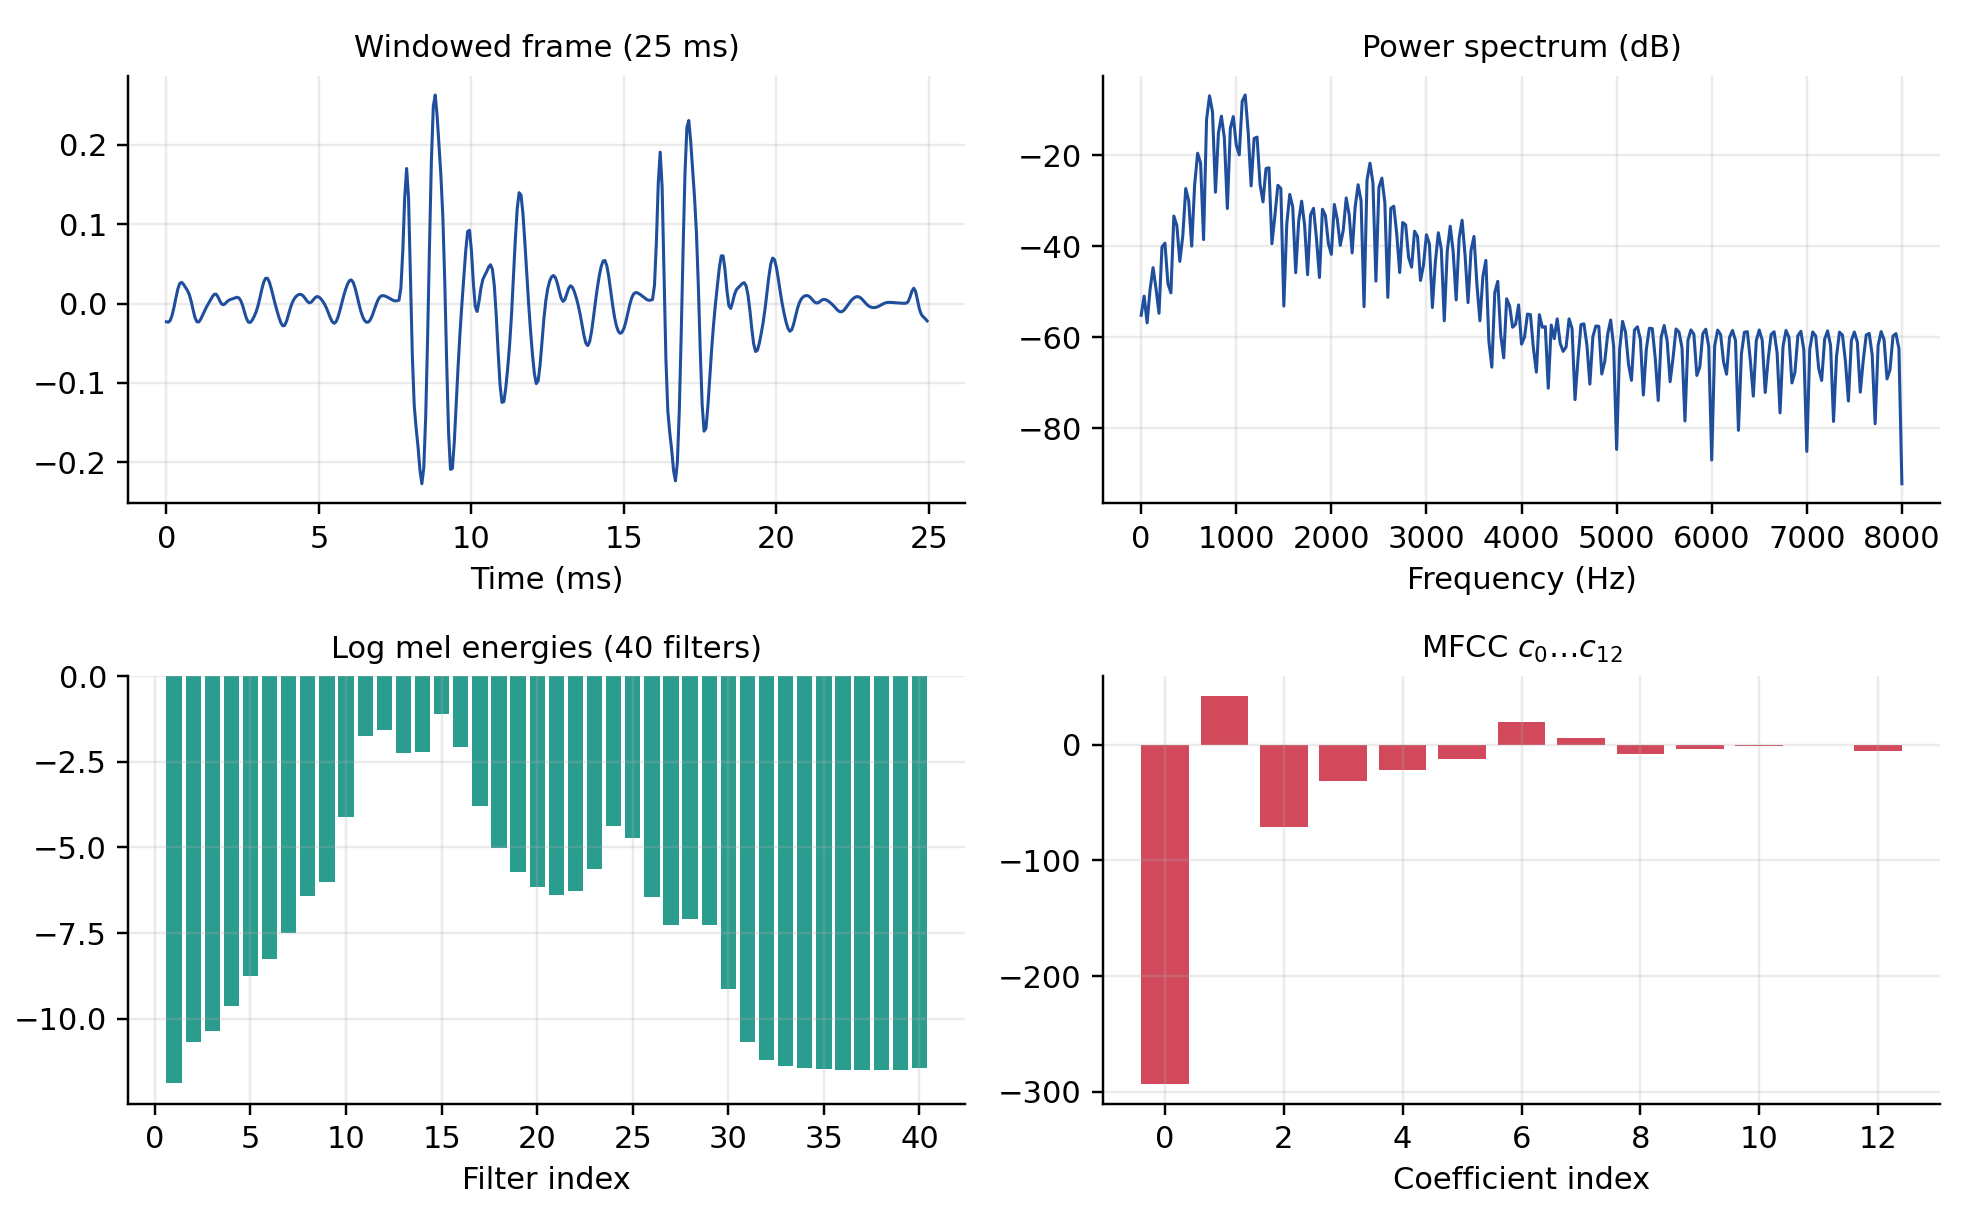
\includegraphics[width=0.95\textwidth]{../assets/figures/ch05-pipeline-demo.png}
  \caption{خروجی مراحل \eng{MFCC} روی یک فریم ۲۵ میلی‌ثانیه‌ای از یک واکهٔ مصنوعی ($F_0=120$ هرتز): فریم پنجره‌گذاری‌شده، طیف توان، لگاریتم انرژی ۴۰ فیلتر مل و ۱۳ ضریب \eng{MFCC} (ضریب $c_0$ بزرگ و منفی است چون به لگاریتم انرژی کلی بستگی دارد). مراحل بالا انبوهی از جزئیات طیف را به ۱۳ عدد تبدیل می‌کنند. (شکل افزوده)}
  \label{fig:pipedemo}
\end{figure}

\begin{figure}[htbp]
  \centering
  \fbox{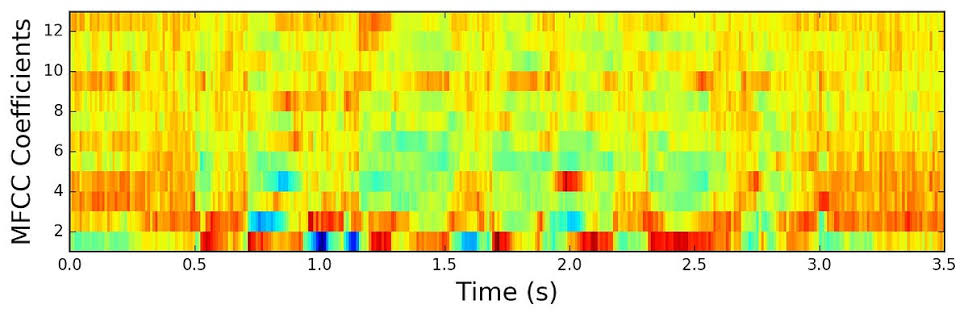
\includegraphics[width=0.85\textwidth]{../assets/figures/ch05-mfcc-matrix.png}}
  \caption{نمایش ماتریسی \eng{MFCC}: محور افقی زمان و محور عمودی شمارهٔ ضریب (۱ تا ۱۳) است؛ رنگ مقدار هر ضریب را در هر فریم نشان می‌دهد. \textit{(برگرفته از تختهٔ کلاس)}}
  \label{fig:mfccmat}
\end{figure}

\boardfigure{0.6}{ch05-board-overview.png}{خلاصهٔ تختهٔ جلسه: سه مرحلهٔ بانک فیلتر مل، لگاریتم و \eng{DCT}؛ در هر مرحله «مسئله» (سمت چپ) و «راه‌حل» (سمت راست) نوشته شده است. در بخش پایین، ماتریس \eng{MFCC} نمایش داده شده است.}

\begin{exambox}{جمع‌بندی سه مسئله و راه‌حل در تخته}
\begin{enumerate}
  \item \textbf{بانک فیلتر مل}: مسئلهٔ ادراک غیرخطی فرکانس $\Leftarrow$ مقیاس مل (نگاشت غیرخطی که فرکانس‌های فیزیکی را «فشرده» می‌کند).
  \item \textbf{لگاریتم}: مسئلهٔ ادراک غیرخطی بلندی (۱۰۰ برابر بلندتر را فقط چند برابر بلندتر حس می‌کنیم) $\Leftarrow$ لگاریتم از انرژی مل.
  \item \textbf{\eng{DCT}}: مسئلهٔ ۴۰ عدد بسیار شبیه و تکراری $\Leftarrow$ \eng{DCT} و برداشتن ۱۲ تا ۱۳ ضریب اول.
\end{enumerate}
\end{exambox}

%====================================================================
\section{کاربردهای MFCC}
%====================================================================

پس از استخراج، به‌جای نمایش‌های حجیم‌تر سیگنال می‌توان از ماتریس \eng{MFCC} (برای هر فریم زمانی یک بردار ضریب) برای تحلیل و مقایسهٔ گفتار استفاده کرد. کاربردهایی که در کلاس مطرح شد:
\begin{itemize}
  \item \textbf{مقایسهٔ سیگنال‌ها}: می‌توان \eng{MFCC} دو سیگنال را استخراج و شباهتشان را (مثلاً با هم‌بستگی، \eng{Correlation}) سنجید.
  \item \textbf{تحلیل صدای سرفه}: اگر دو گروه نمونه داشته باشیم، مثلاً سرفهٔ افراد مبتلا به یک بیماری تنفسی (مانند کووید-۱۹) و سرفهٔ سایرین، می‌توان از هر نمونه \eng{MFCC} گرفت و الگوها را مقایسه یا یک طبقه‌بند آموزش داد. این مثال نشان می‌دهد \eng{MFCC} فقط به تشخیص کلمات محدود نیست.
  \item \textbf{تبدیل گفتار به متن}: به‌جای دادن موج خام، ویژگی‌های آکوستیکی مانند \eng{MFCC} به مدل داده می‌شود. اگر ویژگی دیگری مانند \eng{pitch} لازم باشد، می‌توان آن را جداگانه استخراج کرد؛ چون \eng{MFCC} جایگزین همهٔ ویژگی‌ها نیست.
\end{itemize}

\begin{warningbox}{هشدار دربارهٔ برداشت‌های سریع}
استخراج \eng{MFCC} یا مشاهدهٔ یک هم‌بستگی به‌تنهایی برای تشخیص بیماری کافی نیست؛ این کار نیازمند داده‌های معتبر و متوازن، آموزش و ارزیابی دقیق مدل است. همچنین مقایسهٔ مستقیم \eng{MFCC} دو سیگنال با طول‌های متفاوت یا سرعت گفتار متفاوت نیازمند هم‌ترازسازی زمانی (مثلاً \eng{DTW}) یا خلاصه‌سازی آماری (میانگین/واریانس ضرایب روی زمان) است.
\end{warningbox}

%====================================================================
\section{MFCC در یادگیری ماشین و یادگیری عمیق}
%====================================================================

\subsection{آیا استخراج MFCC یادگیری ماشین است؟}
استاد تأکید کرد که استخراج \eng{MFCC} در حالت متداول خودش \emph{یک فرایند یادگیری ماشین نیست}: مجموعه‌ای از عملیات ثابت پردازش سیگنال (طیف، بانک فیلتر، لگاریتم، \eng{DCT}، انتخاب ضرایب) با پارامترهای مشخص است و برای محاسبهٔ آن نیازی به آموزش روی داده‌های برچسب‌دار نیست. البته خروجی آن را می‌توان به یک مدل یادگیری ماشین داد.

\subsection{مقایسه با PCA}
دانشجویی پرسید آیا کاهش ویژگی در \eng{MFCC} با \eng{PCA} قابل‌مقایسه است. پاسخ: از نظر هدف کلی (نمایش فشرده‌تر) شباهت دارند، اما مسیر محاسباتی‌شان متفاوت است.

\begin{table}[htbp]
\centering
\caption{مقایسهٔ مفهومی \eng{MFCC} و \eng{PCA} (طبق بحث کلاس).}
\begin{tabular}{p{3.5cm}p{5cm}p{5cm}}
\toprule
\textbf{ویژگی} & \textbf{\eng{MFCC}} & \textbf{\eng{PCA}} \\
\midrule
هدف & استخراج ویژگی آکوستیکی مناسب گفتار & کاهش بُعد و استخراج مؤلفه‌های اصلی \\
نوع روش & زنجیرهٔ تبدیل‌های پردازش سیگنال & روش آماری مبتنی بر داده \\
نیاز به یادگیری از داده & در استخراج متداول، خیر & بله؛ مؤلفه‌ها از داده برآورد می‌شوند \\
ورودی & سیگنال صوتی یا نمایش طیفی & بردارهای ویژگی \\
خروجی & ضرایب کپسترال & مؤلفه‌های اصلی \\
\bottomrule
\end{tabular}
\end{table}

در کلاس مطرح شد که پس از لگاریتم انرژی‌های مل می‌توان به‌جای \eng{DCT} از \eng{PCA} هم استفاده کرد؛ اما آنگاه دیگر با تعریف متداول \eng{MFCC} کار نمی‌کنیم. \eng{MFCC} یک مسیر مشخص و شناخته‌شده برای ویژگی آکوستیکی گفتار است.

\begin{correctionbox}{ارتباط \eng{DCT} و \eng{PCA}}
مقایسهٔ دانشجو نکتهٔ دقیقی را لمس می‌کند: \eng{DCT} را می‌توان تقریبی «ثابت و مستقل از داده» از \eng{PCA} روی لگاریتم انرژی‌های مل دانست (به همان دلیل که در بخش \eng{DCT} گفته شد). تفاوت اصلی این است که \eng{PCA} پایه‌ها را از داده می‌آموزد (و برای هر مجموعه‌داده متفاوت است)، در حالی که پایه‌های \eng{DCT} ثابت‌اند.
\end{correctionbox}

\subsection{MFCC در مدل‌های یادگیری عمیق}
حتی هنگام استفاده از یادگیری عمیق می‌توان \eng{MFCC} را به مدل داد؛ چون نمایشی ساختاریافته و فشرده از اطلاعات آکوستیکی است و مدل را از مواجهه با موج خام بی‌نیاز می‌کند. انتخاب میان موج خام، طیف، \eng{MFCC} و نمایش‌های دیگر به مسئله و عملکرد تجربی بستگی دارد.

\begin{correctionbox}{روند امروز: \eng{log-mel} به‌جای \eng{MFCC} در شبکه‌های عمیق}
در عمل، مدل‌های عصبی امروزی (از جمله بسیاری از سامانه‌های تشخیص گفتار مانند \eng{Whisper}) بیشتر از \emph{لگاریتم انرژی‌های مل} (\eng{log-mel filterbank} یا \eng{log-mel spectrogram}) استفاده می‌کنند و مرحلهٔ \eng{DCT} را حذف می‌کنند، چون شبکه خودش می‌تواند هم‌بستگی‌ها را بیاموزد، و \eng{DCT} ترتیب فرکانسی (مناسب برای لایه‌های کانولوشنی) را به هم می‌ریزد. برخی مدل‌های جدید (مانند \eng{wav2vec 2.0}) نیز مستقیماً از موج خام شروع می‌کنند. \eng{MFCC} همچنان در مدل‌های کلاسیک (\eng{GMM-HMM})، مدل‌های سبک و داده‌های کم کاربرد دارد.
\end{correctionbox}

\begin{table}[htbp]
\centering
\caption{نمایش‌های ورودی رایج برای سامانه‌های گفتاری (جمع‌بندی افزوده).}
\begin{tabular}{p{3.2cm}p{3cm}p{6.5cm}}
\toprule
\textbf{نمایش} & \textbf{بُعد تقریبی هر فریم} & \textbf{کاربرد معمول} \\
\midrule
موج خام & ۱۶۰ نمونه در هر ۱۰ میلی‌ثانیه & مدل‌های سرتاسری جدید (\eng{wav2vec 2.0}) \\
طیف‌نگاره (\eng{STFT}) & ۲۵۷ & تحلیل، برخی مدل‌های بهبود گفتار \\
\eng{log-mel} & ۴۰ تا ۱۲۸ & بیشتر شبکه‌های عصبی تشخیص گفتار \\
\eng{MFCC} (+ دلتا) & ۱۳ (۳۹) & مدل‌های کلاسیک، سامانه‌های سبک \\
\bottomrule
\end{tabular}
\end{table}

%====================================================================
\section{جمع‌بندی}
%====================================================================

در این جلسه تحلیل آکوستیکی صرف را به سمت ویژگی‌هایی که با شنوایی انسان سازگارند گسترش دادیم. گوش فرکانس‌ها را غیرخطی درک می‌کند (نقشهٔ تونوتوپیک حلزون، تفکیک بیشتر در فرکانس‌های بم) و شدت را نیز غیرخطی درک می‌کند. برای مدل‌کردن اولی از مقیاس مل و بانک فیلتر مثلثی هم‌پوشان با عرض‌های رشدیابنده استفاده کردیم و برای دومی از لگاریتم. سپس چون ۴۰ انرژی لگاریتمی مل بسیار هم‌بسته‌اند، با \eng{DCT} آن‌ها را به ضرایب کپسترال تبدیل و ۱۲ تا ۱۳ ضریب اول را نگه داشتیم. زنجیرهٔ مفهومی جلسه:
\[
\text{\lr{Speech Signal}}\to\text{\lr{Spectrum}}\to\text{\lr{Mel Filters}}\to\log\to\text{\lr{DCT}}\to\text{\lr{MFCC}} .
\]
نتیجهٔ اصلی: در \eng{MFCC} به‌جای استفاده از همهٔ اطلاعات طیفی، نمایشی فشرده و مناسب گفتار می‌سازیم که ویژگی‌های ادراکی گوش انسان در طراحی آن لحاظ شده است. ادامهٔ بررسی جزئیات برخی ویژگی‌های صوتی (مانند نحوهٔ محاسبهٔ کانتور \eng{pitch}) به جلسه‌های بعد موکول شد.

\begin{exambox}{نکات مهم برای مرور و امتحان}
\begin{enumerate}
  \item تفاوت فرکانس فیزیکی ($F_0$) با ادراک زیر و بمی (\eng{Pitch}) را بدانید.
  \item تفاوت شدت فیزیکی با بلندی ادراک‌شده را توضیح دهید.
  \item نقشهٔ تونوتوپیک حلزون (قاعده $\Leftrightarrow$ فرکانس بالا، رأس $\Leftrightarrow$ فرکانس پایین) و پیامد آن (کم‌شنوایی فرکانس بالا با سن) را بشناسید.
  \item توضیح دهید چرا ادراک انسان از تغییرات فرکانس خطی نیست (مثال ۱۰۰ تا ۲۰۰ در برابر ۵۱۰۰ تا ۵۲۰۰ هرتز).
  \item دلیل استفاده از مقیاس مل و بانک فیلتر مثلثی را بدانید؛ فرمول $m=2595\log_{10}(1+f/700)$.
  \item بدانید چرا عرض فیلترهای مل در فرکانس‌های بالا بیشتر می‌شود.
  \item مفهوم هم‌پوشانی فیلترها و وزن‌دهی مثلثی را توضیح دهید و بتوانید خروجی یک فیلتر را محاسبه کنید (مثال $M_1=13$).
  \item دلیل لگاریتم از انرژی فیلترهای مل را توضیح دهید.
  \item نقش \eng{DCT} (کاهش هم‌بستگی و فشرده‌سازی) و دلیل نگه‌داشتن ۱۲ یا ۱۳ ضریب را بدانید.
  \item مسیر استخراج \eng{MFCC} را از سیگنال تا ضرایب نهایی شرح دهید.
  \item بدانید تعداد فیلترها (حدود ۴۰) و تعداد ضرایب (۱۲ یا ۱۳) ابرپارامترند و ثابت و اجباری نیستند.
  \item تفاوت \eng{MFCC} (زنجیرهٔ ثابت پردازش سیگنال) با \eng{PCA} (یادگیری از داده) را بدانید.
  \item معنای واژهٔ کپستروم (جابه‌جایی حروف \eng{Spectrum}) و ارتباط آن با «طیفِ طیف» را بدانید.
\end{enumerate}
\end{exambox}
